\documentclass[twoside]{book}

% Packages required by doxygen
\usepackage{fixltx2e}
\usepackage{calc}
\usepackage{doxygen}
\usepackage[export]{adjustbox} % also loads graphicx
\usepackage{graphicx}
\usepackage[utf8]{inputenc}
\usepackage{makeidx}
\usepackage{multicol}
\usepackage{multirow}
\PassOptionsToPackage{warn}{textcomp}
\usepackage{textcomp}
\usepackage[nointegrals]{wasysym}
\usepackage[table]{xcolor}

% Font selection
\usepackage[T1]{fontenc}
\usepackage[scaled=.90]{helvet}
\usepackage{courier}
\usepackage{amssymb}
\usepackage{sectsty}
\renewcommand{\familydefault}{\sfdefault}
\allsectionsfont{%
  \fontseries{bc}\selectfont%
  \color{darkgray}%
}
\renewcommand{\DoxyLabelFont}{%
  \fontseries{bc}\selectfont%
  \color{darkgray}%
}
\newcommand{\+}{\discretionary{\mbox{\scriptsize$\hookleftarrow$}}{}{}}

% Page & text layout
\usepackage{geometry}
\geometry{%
  a4paper,%
  top=2.5cm,%
  bottom=2.5cm,%
  left=2.5cm,%
  right=2.5cm%
}
\tolerance=750
\hfuzz=15pt
\hbadness=750
\setlength{\emergencystretch}{15pt}
\setlength{\parindent}{0cm}
\setlength{\parskip}{3ex plus 2ex minus 2ex}
\makeatletter
\renewcommand{\paragraph}{%
  \@startsection{paragraph}{4}{0ex}{-1.0ex}{1.0ex}{%
    \normalfont\normalsize\bfseries\SS@parafont%
  }%
}
\renewcommand{\subparagraph}{%
  \@startsection{subparagraph}{5}{0ex}{-1.0ex}{1.0ex}{%
    \normalfont\normalsize\bfseries\SS@subparafont%
  }%
}
\makeatother

% Headers & footers
\usepackage{fancyhdr}
\pagestyle{fancyplain}
\fancyhead[LE]{\fancyplain{}{\bfseries\thepage}}
\fancyhead[CE]{\fancyplain{}{}}
\fancyhead[RE]{\fancyplain{}{\bfseries\leftmark}}
\fancyhead[LO]{\fancyplain{}{\bfseries\rightmark}}
\fancyhead[CO]{\fancyplain{}{}}
\fancyhead[RO]{\fancyplain{}{\bfseries\thepage}}
\fancyfoot[LE]{\fancyplain{}{}}
\fancyfoot[CE]{\fancyplain{}{}}
\fancyfoot[RE]{\fancyplain{}{\bfseries\scriptsize Generated by Doxygen }}
\fancyfoot[LO]{\fancyplain{}{\bfseries\scriptsize Generated by Doxygen }}
\fancyfoot[CO]{\fancyplain{}{}}
\fancyfoot[RO]{\fancyplain{}{}}
\renewcommand{\footrulewidth}{0.4pt}
\renewcommand{\chaptermark}[1]{%
  \markboth{#1}{}%
}
\renewcommand{\sectionmark}[1]{%
  \markright{\thesection\ #1}%
}

% Indices & bibliography
\usepackage{natbib}
\usepackage[titles]{tocloft}
\setcounter{tocdepth}{3}
\setcounter{secnumdepth}{5}
\makeindex

% Custom commands
\newcommand{\clearemptydoublepage}{%
  \newpage{\pagestyle{empty}\cleardoublepage}%
}

\usepackage{caption}
\captionsetup{labelsep=space,justification=centering,font={bf},singlelinecheck=off,skip=4pt,position=top}

%===== C O N T E N T S =====

\begin{document}

% Titlepage & ToC
\pagenumbering{alph}
\begin{titlepage}
\vspace*{7cm}
\begin{center}%
{\Large k-\/means in native C++ \\[1ex]\large v1.\+0 }\\
\vspace*{1cm}
{\large Generated by Doxygen 1.8.14}\\
\end{center}
\end{titlepage}
\clearemptydoublepage
\pagenumbering{roman}
\tableofcontents
\clearemptydoublepage
\pagenumbering{arabic}

%--- Begin generated contents ---
\chapter{R\+E\+A\+D\+ME}
\label{md__r_e_a_d_m_e}
This repo contains the implementation of the k-\/means clustering machine learning algorithm\+:

{\tt https\+://en.\+wikipedia.\+org/wiki/\+K-\/means\+\_\+clustering}

as a native C++ application.

The documentation of the project is in the /doc directory. 
\chapter{Namespace Index}
\section{Namespace List}
Here is a list of all namespaces with brief descriptions\+:\begin{DoxyCompactList}
\item\contentsline{section}{\textbf{ flnc} }{\pageref{namespaceflnc}}{}
\item\contentsline{section}{\textbf{ gf} }{\pageref{namespacegf}}{}
\item\contentsline{section}{\textbf{ mf} }{\pageref{namespacemf}}{}
\end{DoxyCompactList}

\chapter{Class Index}
\section{Class List}
Here are the classes, structs, unions and interfaces with brief descriptions\+:\begin{DoxyCompactList}
\item\contentsline{section}{\textbf{ Cluster} }{\pageref{class_cluster}}{}
\item\contentsline{section}{\textbf{ Kmeans} }{\pageref{class_kmeans}}{}
\item\contentsline{section}{\textbf{ Point} }{\pageref{class_point}}{}
\item\contentsline{section}{\textbf{ Properties\+Parser} }{\pageref{class_properties_parser}}{}
\end{DoxyCompactList}

\chapter{File Index}
\section{File List}
Here is a list of all files with brief descriptions\+:\begin{DoxyCompactList}
\item\contentsline{section}{\textbf{ Cluster.\+cpp} }{\pageref{_cluster_8cpp}}{}
\item\contentsline{section}{\textbf{ Cluster.\+h} }{\pageref{_cluster_8h}}{}
\item\contentsline{section}{\textbf{ Data\+Types.\+h} }{\pageref{_data_types_8h}}{}
\item\contentsline{section}{\textbf{ File\+Func.\+h} }{\pageref{_file_func_8h}}{}
\item\contentsline{section}{\textbf{ Generic\+Func.\+cpp} }{\pageref{_generic_func_8cpp}}{}
\item\contentsline{section}{\textbf{ Generic\+Func.\+h} }{\pageref{_generic_func_8h}}{}
\item\contentsline{section}{\textbf{ Kmeans.\+cpp} }{\pageref{_kmeans_8cpp}}{}
\item\contentsline{section}{\textbf{ Kmeans.\+h} }{\pageref{_kmeans_8h}}{}
\item\contentsline{section}{\textbf{ main.\+cpp} }{\pageref{main_8cpp}}{}
\item\contentsline{section}{\textbf{ Mathematical\+Functions.\+cpp} }{\pageref{_mathematical_functions_8cpp}}{}
\item\contentsline{section}{\textbf{ Mathematical\+Functions.\+h} }{\pageref{_mathematical_functions_8h}}{}
\item\contentsline{section}{\textbf{ Point.\+cpp} }{\pageref{_point_8cpp}}{}
\item\contentsline{section}{\textbf{ Point.\+h} }{\pageref{_point_8h}}{}
\item\contentsline{section}{\textbf{ Properties\+Parser.\+cpp} }{\pageref{_properties_parser_8cpp}}{}
\item\contentsline{section}{\textbf{ Properties\+Parser.\+h} }{\pageref{_properties_parser_8h}}{}
\end{DoxyCompactList}

\chapter{Namespace Documentation}
\section{flnc Namespace Reference}
\label{namespaceflnc}\index{flnc@{flnc}}
\subsection*{Functions}
\begin{DoxyCompactItemize}
\item 
{\footnotesize template$<$typename T\+Y\+PE $>$ }\\void \textbf{ Write\+Vector\+To\+File} (\textbf{ moutput\+\_\+stream} $\ast$Training\+File\+Out, const std\+::vector$<$ T\+Y\+PE $>$ \&vec)
\item 
{\footnotesize template$<$typename T\+Y\+PE $>$ }\\void \textbf{ Write2\+D\+Vector\+To\+File} (\textbf{ moutput\+\_\+stream} $\ast$Training\+File\+Out, const std\+::vector$<$ std\+::vector$<$ T\+Y\+PE $>$ $>$ \&vec)
\item 
{\footnotesize template$<$typename T\+Y\+PE $>$ }\\void \textbf{ Read\+Vector\+From\+File} (\textbf{ minput\+\_\+stream} $\ast$Training\+File\+In, std\+::vector$<$ T\+Y\+PE $>$ \&vec)
\item 
{\footnotesize template$<$typename T\+Y\+PE $>$ }\\void \textbf{ Read2\+D\+Vector\+From\+File} (\textbf{ minput\+\_\+stream} $\ast$Training\+File\+In, std\+::vector$<$ std\+::vector$<$ T\+Y\+PE $>$ $>$ \&vec)
\end{DoxyCompactItemize}


\subsection{Function Documentation}
\mbox{\label{namespaceflnc_a43f11ba9f2a94bcf4e8680f806a54a47}} 
\index{flnc@{flnc}!Read2\+D\+Vector\+From\+File@{Read2\+D\+Vector\+From\+File}}
\index{Read2\+D\+Vector\+From\+File@{Read2\+D\+Vector\+From\+File}!flnc@{flnc}}
\subsubsection{Read2\+D\+Vector\+From\+File()}
{\footnotesize\ttfamily template$<$typename T\+Y\+PE $>$ \\
void flnc\+::\+Read2\+D\+Vector\+From\+File (\begin{DoxyParamCaption}\item[{\textbf{ minput\+\_\+stream} $\ast$}]{Training\+File\+In,  }\item[{std\+::vector$<$ std\+::vector$<$ T\+Y\+PE $>$ $>$ \&}]{vec }\end{DoxyParamCaption})}

Reads a vector of vectors to file. The format of the file must be 
\begin{DoxyCode}
number\_of\_vectors
vector\_size vector\_1st\_element vector\_2nd\_element ...
vector\_size vector\_1st\_element vector\_2nd\_element ...
    ...            ...                ...         ...
\end{DoxyCode}



\begin{DoxyParams}{Parameters}
{\em Training\+File\+In} & the input stream of the file to read the vector from. \\
\hline
{\em vec} & the vector of vectors to be read to file. \\
\hline
\end{DoxyParams}


Definition at line 75 of file File\+Func.\+h.

\mbox{\label{namespaceflnc_a51e2434fe14f26a9d979282b2d6524f5}} 
\index{flnc@{flnc}!Read\+Vector\+From\+File@{Read\+Vector\+From\+File}}
\index{Read\+Vector\+From\+File@{Read\+Vector\+From\+File}!flnc@{flnc}}
\subsubsection{Read\+Vector\+From\+File()}
{\footnotesize\ttfamily template$<$typename T\+Y\+PE $>$ \\
void flnc\+::\+Read\+Vector\+From\+File (\begin{DoxyParamCaption}\item[{\textbf{ minput\+\_\+stream} $\ast$}]{Training\+File\+In,  }\item[{std\+::vector$<$ T\+Y\+PE $>$ \&}]{vec }\end{DoxyParamCaption})}

Reads a vector from file. The format of the file must be 
\begin{DoxyCode}
vector\_size vector\_1st\_element vector\_2nd\_element ...
\end{DoxyCode}



\begin{DoxyParams}{Parameters}
{\em Training\+File\+In} & the input stream of the file to read the vector from. \\
\hline
{\em vec} & the vector to be read to file. \\
\hline
\end{DoxyParams}


Definition at line 55 of file File\+Func.\+h.

\mbox{\label{namespaceflnc_a5ee4b13fe9860b1398a2e2c8d07776c8}} 
\index{flnc@{flnc}!Write2\+D\+Vector\+To\+File@{Write2\+D\+Vector\+To\+File}}
\index{Write2\+D\+Vector\+To\+File@{Write2\+D\+Vector\+To\+File}!flnc@{flnc}}
\subsubsection{Write2\+D\+Vector\+To\+File()}
{\footnotesize\ttfamily template$<$typename T\+Y\+PE $>$ \\
void flnc\+::\+Write2\+D\+Vector\+To\+File (\begin{DoxyParamCaption}\item[{\textbf{ moutput\+\_\+stream} $\ast$}]{Training\+File\+Out,  }\item[{const std\+::vector$<$ std\+::vector$<$ T\+Y\+PE $>$ $>$ \&}]{vec }\end{DoxyParamCaption})}

Writes a vector of vectors to file. The format is\+: 
\begin{DoxyCode}
number\_of\_vectors
vector\_size vector\_1st\_element vector\_2nd\_element ...
vector\_size vector\_1st\_element vector\_2nd\_element ...
    ...            ...                ...         ...
\end{DoxyCode}



\begin{DoxyParams}{Parameters}
{\em Training\+File\+Out} & the output stream of the file to write the vector to. \\
\hline
{\em vec} & the vector of vectors to be written to file. \\
\hline
\end{DoxyParams}


Definition at line 39 of file File\+Func.\+h.

\mbox{\label{namespaceflnc_aa6a517635283780c9142bf6ad194013e}} 
\index{flnc@{flnc}!Write\+Vector\+To\+File@{Write\+Vector\+To\+File}}
\index{Write\+Vector\+To\+File@{Write\+Vector\+To\+File}!flnc@{flnc}}
\subsubsection{Write\+Vector\+To\+File()}
{\footnotesize\ttfamily template$<$typename T\+Y\+PE $>$ \\
void flnc\+::\+Write\+Vector\+To\+File (\begin{DoxyParamCaption}\item[{\textbf{ moutput\+\_\+stream} $\ast$}]{Training\+File\+Out,  }\item[{const std\+::vector$<$ T\+Y\+PE $>$ \&}]{vec }\end{DoxyParamCaption})}

Writes a vector to file. The format is\+: 
\begin{DoxyCode}
vector\_size vector\_1st\_element vector\_2nd\_element ...
\end{DoxyCode}



\begin{DoxyParams}{Parameters}
{\em Training\+File\+Out} & the output stream of the file to write the vector to. \\
\hline
{\em vec} & the vector to be written to file. \\
\hline
\end{DoxyParams}


Definition at line 20 of file File\+Func.\+h.


\section{gf Namespace Reference}
\label{namespacegf}\index{gf@{gf}}
\subsection*{Functions}
\begin{DoxyCompactItemize}
\item 
std\+::string \textbf{ get\+Executable\+Path} ()
\item 
std\+::string \textbf{ get\+Executable\+Path\+And\+Match\+It\+With\+Filename} (std\+::string filename)
\end{DoxyCompactItemize}


\subsection{Function Documentation}
\mbox{\label{namespacegf_ac0f4b1cee2681a53cb7c513c7f9a3b6f}} 
\index{gf@{gf}!get\+Executable\+Path@{get\+Executable\+Path}}
\index{get\+Executable\+Path@{get\+Executable\+Path}!gf@{gf}}
\subsubsection{get\+Executable\+Path()}
{\footnotesize\ttfamily std\+::string gf\+::get\+Executable\+Path (\begin{DoxyParamCaption}{ }\end{DoxyParamCaption})}

Returns the absolute path of the executable\textquotesingle{}s directory. \begin{DoxyReturn}{Returns}
the absolute path of the executable\textquotesingle{}s directory. 
\end{DoxyReturn}


Definition at line 3 of file Generic\+Func.\+cpp.

\mbox{\label{namespacegf_a00f9f0ea9a0804a71cf70c6b1eb158cf}} 
\index{gf@{gf}!get\+Executable\+Path\+And\+Match\+It\+With\+Filename@{get\+Executable\+Path\+And\+Match\+It\+With\+Filename}}
\index{get\+Executable\+Path\+And\+Match\+It\+With\+Filename@{get\+Executable\+Path\+And\+Match\+It\+With\+Filename}!gf@{gf}}
\subsubsection{get\+Executable\+Path\+And\+Match\+It\+With\+Filename()}
{\footnotesize\ttfamily std\+::string gf\+::get\+Executable\+Path\+And\+Match\+It\+With\+Filename (\begin{DoxyParamCaption}\item[{std\+::string}]{filename }\end{DoxyParamCaption})}

Returns the absolute path a file located in the executable\textquotesingle{}s directory. 
\begin{DoxyParams}{Parameters}
{\em file\+Name} & the name of the file (e.\+g., file.\+txt) \\
\hline
\end{DoxyParams}
\begin{DoxyReturn}{Returns}
the absolute path of the file 
\end{DoxyReturn}


Definition at line 10 of file Generic\+Func.\+cpp.


\section{mf Namespace Reference}
\label{namespacemf}\index{mf@{mf}}
\subsection*{Functions}
\begin{DoxyCompactItemize}
\item 
size\+\_\+t \textbf{ min\+Size} (\textbf{ Point} \&p, \textbf{ Point} \&q)
\item 
double \textbf{ mean} (\textbf{ Point} \&p)
\item 
double \textbf{ st\+Dev} (\textbf{ Point} \&p)
\item 
double \textbf{ euclidean\+Distance} (\textbf{ Point} \&p, \textbf{ Point} \&q)
\item 
double \textbf{ euclidean\+Distance\+Squared} (\textbf{ Point} \&p, \textbf{ Point} \&q)
\item 
double \textbf{ manhattan\+Distance} (\textbf{ Point} \&p, \textbf{ Point} \&q)
\item 
double \textbf{ chebyshev\+Distance} (\textbf{ Point} \&p, \textbf{ Point} \&q)
\item 
double \textbf{ bray\+Curtis\+Distance} (\textbf{ Point} \&p, \textbf{ Point} \&q)
\item 
double \textbf{ canberra\+Distance} (\textbf{ Point} \&p, \textbf{ Point} \&q)
\item 
double \textbf{ pearson\+Correlation} (\textbf{ Point} \&p, \textbf{ Point} \&q)
\item 
double \textbf{ cosine\+Similarity} (\textbf{ Point} \&p, \textbf{ Point} \&q)
\item 
double \textbf{ dot} (\textbf{ Point} \&p, \textbf{ Point} \&q)
\end{DoxyCompactItemize}


\subsection{Function Documentation}
\mbox{\label{namespacemf_a53713d1a18fc6069e8da721e56dda3d1}} 
\index{mf@{mf}!bray\+Curtis\+Distance@{bray\+Curtis\+Distance}}
\index{bray\+Curtis\+Distance@{bray\+Curtis\+Distance}!mf@{mf}}
\subsubsection{bray\+Curtis\+Distance()}
{\footnotesize\ttfamily double mf\+::bray\+Curtis\+Distance (\begin{DoxyParamCaption}\item[{\textbf{ Point} \&}]{p,  }\item[{\textbf{ Point} \&}]{q }\end{DoxyParamCaption})}

Computes the Bray–\+Curtis distance between two \doxyref{Point}{p.}{class_point} objects. {\tt https\+://en.\+wikipedia.\+org/wiki/\+Bray\%\+E2\%80\%93\+Curtis\+\_\+dissimilarity} 
\begin{DoxyParams}{Parameters}
{\em p} & the first \doxyref{Point}{p.}{class_point}. \\
\hline
{\em q} & the second \doxyref{Point}{p.}{class_point}.  the Bray–\+Curtis distance. \\
\hline
\end{DoxyParams}


Definition at line 68 of file Mathematical\+Functions.\+cpp.

\mbox{\label{namespacemf_a000039a6817d1eaab151f74651c5fac4}} 
\index{mf@{mf}!canberra\+Distance@{canberra\+Distance}}
\index{canberra\+Distance@{canberra\+Distance}!mf@{mf}}
\subsubsection{canberra\+Distance()}
{\footnotesize\ttfamily double mf\+::canberra\+Distance (\begin{DoxyParamCaption}\item[{\textbf{ Point} \&}]{p,  }\item[{\textbf{ Point} \&}]{q }\end{DoxyParamCaption})}

Computes the Canberra distance between two \doxyref{Point}{p.}{class_point} objects. {\tt https\+://en.\+wikipedia.\+org/wiki/\+Canberra\+\_\+distance} 
\begin{DoxyParams}{Parameters}
{\em p} & the first \doxyref{Point}{p.}{class_point}. \\
\hline
{\em q} & the second \doxyref{Point}{p.}{class_point}.  the Canberra distance. \\
\hline
\end{DoxyParams}


Definition at line 82 of file Mathematical\+Functions.\+cpp.

\mbox{\label{namespacemf_aff2481aba46c30ed52226097357bb526}} 
\index{mf@{mf}!chebyshev\+Distance@{chebyshev\+Distance}}
\index{chebyshev\+Distance@{chebyshev\+Distance}!mf@{mf}}
\subsubsection{chebyshev\+Distance()}
{\footnotesize\ttfamily double mf\+::chebyshev\+Distance (\begin{DoxyParamCaption}\item[{\textbf{ Point} \&}]{p,  }\item[{\textbf{ Point} \&}]{q }\end{DoxyParamCaption})}

Computes the Chebyshev distance between two \doxyref{Point}{p.}{class_point} objects. {\tt https\+://en.\+wikipedia.\+org/wiki/\+Chebyshev\+\_\+distance} 
\begin{DoxyParams}{Parameters}
{\em p} & the first \doxyref{Point}{p.}{class_point}. \\
\hline
{\em q} & the second \doxyref{Point}{p.}{class_point}.  the Chebyshev distance. \\
\hline
\end{DoxyParams}


Definition at line 53 of file Mathematical\+Functions.\+cpp.

\mbox{\label{namespacemf_ad3df0be2c20cff9d29cc6b3c550fd467}} 
\index{mf@{mf}!cosine\+Similarity@{cosine\+Similarity}}
\index{cosine\+Similarity@{cosine\+Similarity}!mf@{mf}}
\subsubsection{cosine\+Similarity()}
{\footnotesize\ttfamily double mf\+::cosine\+Similarity (\begin{DoxyParamCaption}\item[{\textbf{ Point} \&}]{p,  }\item[{\textbf{ Point} \&}]{q }\end{DoxyParamCaption})}

Computes the cosine similarity between two \doxyref{Point}{p.}{class_point} objects. {\tt https\+://en.\+wikipedia.\+org/wiki/\+Cosine\+\_\+similarity} 
\begin{DoxyParams}{Parameters}
{\em p} & the first \doxyref{Point}{p.}{class_point}. \\
\hline
{\em q} & the second \doxyref{Point}{p.}{class_point}.  the cosine similarity. \\
\hline
\end{DoxyParams}


Definition at line 111 of file Mathematical\+Functions.\+cpp.

\mbox{\label{namespacemf_a0a73292f72b80df3a0c6b970e2ca4be6}} 
\index{mf@{mf}!dot@{dot}}
\index{dot@{dot}!mf@{mf}}
\subsubsection{dot()}
{\footnotesize\ttfamily double mf\+::dot (\begin{DoxyParamCaption}\item[{\textbf{ Point} \&}]{p,  }\item[{\textbf{ Point} \&}]{q }\end{DoxyParamCaption})}

Computes the dot product between two \doxyref{Point}{p.}{class_point} objects. {\tt https\+://en.\+wikipedia.\+org/wiki/\+Dot\+\_\+product} 
\begin{DoxyParams}{Parameters}
{\em p} & the first \doxyref{Point}{p.}{class_point}. \\
\hline
{\em q} & the second \doxyref{Point}{p.}{class_point}.  the dot product. \\
\hline
\end{DoxyParams}


Definition at line 128 of file Mathematical\+Functions.\+cpp.

\mbox{\label{namespacemf_a40500525d65df0f162783485b005a17c}} 
\index{mf@{mf}!euclidean\+Distance@{euclidean\+Distance}}
\index{euclidean\+Distance@{euclidean\+Distance}!mf@{mf}}
\subsubsection{euclidean\+Distance()}
{\footnotesize\ttfamily double mf\+::euclidean\+Distance (\begin{DoxyParamCaption}\item[{\textbf{ Point} \&}]{p,  }\item[{\textbf{ Point} \&}]{q }\end{DoxyParamCaption})}

Computes the Euclidean distance between two \doxyref{Point}{p.}{class_point} objects. {\tt https\+://en.\+wikipedia.\+org/wiki/\+Euclidean\+\_\+distance} 
\begin{DoxyParams}{Parameters}
{\em p} & the first \doxyref{Point}{p.}{class_point}. \\
\hline
{\em q} & the second \doxyref{Point}{p.}{class_point}.  the Euclidean distance. \\
\hline
\end{DoxyParams}


Definition at line 25 of file Mathematical\+Functions.\+cpp.

\mbox{\label{namespacemf_a18bfb051b8501f49ad1ce7910cf5fa4e}} 
\index{mf@{mf}!euclidean\+Distance\+Squared@{euclidean\+Distance\+Squared}}
\index{euclidean\+Distance\+Squared@{euclidean\+Distance\+Squared}!mf@{mf}}
\subsubsection{euclidean\+Distance\+Squared()}
{\footnotesize\ttfamily double mf\+::euclidean\+Distance\+Squared (\begin{DoxyParamCaption}\item[{\textbf{ Point} \&}]{p,  }\item[{\textbf{ Point} \&}]{q }\end{DoxyParamCaption})}

Computes the squared Euclidean distance between two \doxyref{Point}{p.}{class_point} objects. {\tt https\+://en.\+wikipedia.\+org/wiki/\+Euclidean\+\_\+distance} 
\begin{DoxyParams}{Parameters}
{\em p} & the first \doxyref{Point}{p.}{class_point}. \\
\hline
{\em q} & the second \doxyref{Point}{p.}{class_point}.  the squared Euclidean distance. \\
\hline
\end{DoxyParams}


Definition at line 37 of file Mathematical\+Functions.\+cpp.

\mbox{\label{namespacemf_a040ab6b23a68d7a4c2f818c1eae58644}} 
\index{mf@{mf}!manhattan\+Distance@{manhattan\+Distance}}
\index{manhattan\+Distance@{manhattan\+Distance}!mf@{mf}}
\subsubsection{manhattan\+Distance()}
{\footnotesize\ttfamily double mf\+::manhattan\+Distance (\begin{DoxyParamCaption}\item[{\textbf{ Point} \&}]{p,  }\item[{\textbf{ Point} \&}]{q }\end{DoxyParamCaption})}

Computes the Manhattan (or taxicab) distance between two \doxyref{Point}{p.}{class_point} objects. {\tt https\+://en.\+wikipedia.\+org/wiki/\+Taxicab\+\_\+geometry} 
\begin{DoxyParams}{Parameters}
{\em p} & the first \doxyref{Point}{p.}{class_point}. \\
\hline
{\em q} & the second \doxyref{Point}{p.}{class_point}.  the Manhattan distance. \\
\hline
\end{DoxyParams}


Definition at line 42 of file Mathematical\+Functions.\+cpp.

\mbox{\label{namespacemf_ad29e1be602cf1426190438ba4a978886}} 
\index{mf@{mf}!mean@{mean}}
\index{mean@{mean}!mf@{mf}}
\subsubsection{mean()}
{\footnotesize\ttfamily double mf\+::mean (\begin{DoxyParamCaption}\item[{\textbf{ Point} \&}]{p }\end{DoxyParamCaption})}

Returns the mean value of a \doxyref{Point}{p.}{class_point}. \begin{DoxyReturn}{Returns}
the mean value. 
\end{DoxyReturn}


Definition at line 11 of file Mathematical\+Functions.\+cpp.

\mbox{\label{namespacemf_aacf640ab87407a419a237ff36d0c0c09}} 
\index{mf@{mf}!min\+Size@{min\+Size}}
\index{min\+Size@{min\+Size}!mf@{mf}}
\subsubsection{min\+Size()}
{\footnotesize\ttfamily size\+\_\+t mf\+::min\+Size (\begin{DoxyParamCaption}\item[{\textbf{ Point} \&}]{p,  }\item[{\textbf{ Point} \&}]{q }\end{DoxyParamCaption})}

Returns the minimum of the sizes of two \doxyref{Point}{p.}{class_point} objects. \begin{DoxyReturn}{Returns}
the minimum of the sizes. 
\end{DoxyReturn}


Definition at line 3 of file Mathematical\+Functions.\+cpp.

\mbox{\label{namespacemf_a00075eb9a854aee2323bf1f9e51cf1fa}} 
\index{mf@{mf}!pearson\+Correlation@{pearson\+Correlation}}
\index{pearson\+Correlation@{pearson\+Correlation}!mf@{mf}}
\subsubsection{pearson\+Correlation()}
{\footnotesize\ttfamily double mf\+::pearson\+Correlation (\begin{DoxyParamCaption}\item[{\textbf{ Point} \&}]{p,  }\item[{\textbf{ Point} \&}]{q }\end{DoxyParamCaption})}

Computes the Pearson correlation coefficient between two \doxyref{Point}{p.}{class_point} objects. {\tt https\+://en.\+wikipedia.\+org/wiki/\+Pearson\+\_\+correlation\+\_\+coefficient} 
\begin{DoxyParams}{Parameters}
{\em p} & the first \doxyref{Point}{p.}{class_point}. \\
\hline
{\em q} & the second \doxyref{Point}{p.}{class_point}.  the Pearson correlation coefficient. \\
\hline
\end{DoxyParams}


Definition at line 93 of file Mathematical\+Functions.\+cpp.

\mbox{\label{namespacemf_a7b665e7f861360232bc6ff8b4ab53b79}} 
\index{mf@{mf}!st\+Dev@{st\+Dev}}
\index{st\+Dev@{st\+Dev}!mf@{mf}}
\subsubsection{st\+Dev()}
{\footnotesize\ttfamily double mf\+::st\+Dev (\begin{DoxyParamCaption}\item[{\textbf{ Point} \&}]{p }\end{DoxyParamCaption})}

Returns the standard deviation value of a \doxyref{Point}{p.}{class_point}. \begin{DoxyReturn}{Returns}
the standard deviation value. 
\end{DoxyReturn}


Definition at line 16 of file Mathematical\+Functions.\+cpp.


\chapter{Class Documentation}
\section{Cluster Class Reference}
\label{class_cluster}\index{Cluster@{Cluster}}


{\ttfamily \#include $<$Cluster.\+h$>$}



Collaboration diagram for Cluster\+:\nopagebreak
\begin{figure}[H]
\begin{center}
\leavevmode
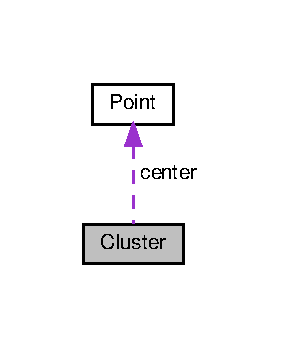
\includegraphics[width=135pt]{class_cluster__coll__graph}
\end{center}
\end{figure}
\subsection*{Public Member Functions}
\begin{DoxyCompactItemize}
\item 
\textbf{ Cluster} (\textbf{ Point} c, int id)
\item 
\textbf{ $\sim$\+Cluster} ()
\item 
void \textbf{ set\+ID} (int ID)
\item 
int \textbf{ get\+ID} () const
\item 
void \textbf{ set\+Center} (\textbf{ Point} \&\textbf{ center})
\item 
\textbf{ Point} \textbf{ get\+Center} ()
\item 
void \textbf{ set\+Points\+To\+Cluster} (\textbf{ Point} $\ast$p)
\item 
size\+\_\+t \textbf{ get\+Num\+Of\+Points\+In\+Cluster} ()
\item 
\textbf{ Point} $\ast$ \textbf{ get\+Point\+Of\+Cluster} (size\+\_\+t index)
\item 
void \textbf{ clear\+Points\+Of\+Cluster} ()
\item 
bool \textbf{ operator==} (\textbf{ Cluster} \&c)
\item 
bool \textbf{ operator$<$} (\textbf{ Cluster} \&c)
\item 
void \textbf{ print\+Centroid\+In\+Console} ()
\item 
void \textbf{ print\+Allocation\+In\+Console} ()
\item 
void \textbf{ write\+Centroid\+To\+File} (std\+::ostream \&out)
\item 
void \textbf{ write\+Allocation\+To\+File} (std\+::ostream \&out)
\end{DoxyCompactItemize}
\subsection*{Public Attributes}
\begin{DoxyCompactItemize}
\item 
std\+::vector$<$ \textbf{ Point} $\ast$ $>$ \textbf{ points\+Of\+Cluster}
\item 
\textbf{ Point} \textbf{ center}
\end{DoxyCompactItemize}


\subsection{Detailed Description}


Definition at line 6 of file Cluster.\+h.



\subsection{Constructor \& Destructor Documentation}
\mbox{\label{class_cluster_a5e07ba3b4772eb29eeac0095eef3cd3a}} 
\index{Cluster@{Cluster}!Cluster@{Cluster}}
\index{Cluster@{Cluster}!Cluster@{Cluster}}
\subsubsection{Cluster()}
{\footnotesize\ttfamily Cluster\+::\+Cluster (\begin{DoxyParamCaption}\item[{\textbf{ Point}}]{c,  }\item[{int}]{id }\end{DoxyParamCaption})}

Constructor. 

Definition at line 3 of file Cluster.\+cpp.

\mbox{\label{class_cluster_a4bddfc88ac859610acab15dd12851b58}} 
\index{Cluster@{Cluster}!````~Cluster@{$\sim$\+Cluster}}
\index{````~Cluster@{$\sim$\+Cluster}!Cluster@{Cluster}}
\subsubsection{$\sim$\+Cluster()}
{\footnotesize\ttfamily Cluster\+::$\sim$\+Cluster (\begin{DoxyParamCaption}{ }\end{DoxyParamCaption})}

Destructor. 

Definition at line 7 of file Cluster.\+cpp.



\subsection{Member Function Documentation}
\mbox{\label{class_cluster_afa46912376ac9690ee946612ddc99c76}} 
\index{Cluster@{Cluster}!clear\+Points\+Of\+Cluster@{clear\+Points\+Of\+Cluster}}
\index{clear\+Points\+Of\+Cluster@{clear\+Points\+Of\+Cluster}!Cluster@{Cluster}}
\subsubsection{clear\+Points\+Of\+Cluster()}
{\footnotesize\ttfamily void Cluster\+::clear\+Points\+Of\+Cluster (\begin{DoxyParamCaption}{ }\end{DoxyParamCaption})}

Deletes all points of the \doxyref{Cluster}{p.}{class_cluster}. 

Definition at line 53 of file Cluster.\+cpp.

\mbox{\label{class_cluster_a72b992c37dc0792e84dbe5ac2d89bbbe}} 
\index{Cluster@{Cluster}!get\+Center@{get\+Center}}
\index{get\+Center@{get\+Center}!Cluster@{Cluster}}
\subsubsection{get\+Center()}
{\footnotesize\ttfamily \textbf{ Point} Cluster\+::get\+Center (\begin{DoxyParamCaption}{ }\end{DoxyParamCaption})}

Returns the center of the \doxyref{Cluster}{p.}{class_cluster}. \begin{DoxyReturn}{Returns}
the center (i.\+e., a \doxyref{Point}{p.}{class_point} object) of the \doxyref{Cluster}{p.}{class_cluster}. 
\end{DoxyReturn}


Definition at line 30 of file Cluster.\+cpp.

\mbox{\label{class_cluster_a7e3843eaa486b9dd28de25a7c9f4e1f9}} 
\index{Cluster@{Cluster}!get\+ID@{get\+ID}}
\index{get\+ID@{get\+ID}!Cluster@{Cluster}}
\subsubsection{get\+I\+D()}
{\footnotesize\ttfamily int Cluster\+::get\+ID (\begin{DoxyParamCaption}{ }\end{DoxyParamCaption}) const}

Returns the ID of the \doxyref{Cluster}{p.}{class_cluster}. \begin{DoxyReturn}{Returns}
the ID of the \doxyref{Cluster}{p.}{class_cluster}. 
\end{DoxyReturn}


Definition at line 20 of file Cluster.\+cpp.

\mbox{\label{class_cluster_a937233153e5610b9e8d91815e3a43b5e}} 
\index{Cluster@{Cluster}!get\+Num\+Of\+Points\+In\+Cluster@{get\+Num\+Of\+Points\+In\+Cluster}}
\index{get\+Num\+Of\+Points\+In\+Cluster@{get\+Num\+Of\+Points\+In\+Cluster}!Cluster@{Cluster}}
\subsubsection{get\+Num\+Of\+Points\+In\+Cluster()}
{\footnotesize\ttfamily size\+\_\+t Cluster\+::get\+Num\+Of\+Points\+In\+Cluster (\begin{DoxyParamCaption}{ }\end{DoxyParamCaption})}

Returns the number of points in the \doxyref{Cluster}{p.}{class_cluster}. \begin{DoxyReturn}{Returns}
the number of points in the \doxyref{Cluster}{p.}{class_cluster}. 
\end{DoxyReturn}


Definition at line 40 of file Cluster.\+cpp.

\mbox{\label{class_cluster_a77c17b4532c831f5c9c3ef9fdc4f3822}} 
\index{Cluster@{Cluster}!get\+Point\+Of\+Cluster@{get\+Point\+Of\+Cluster}}
\index{get\+Point\+Of\+Cluster@{get\+Point\+Of\+Cluster}!Cluster@{Cluster}}
\subsubsection{get\+Point\+Of\+Cluster()}
{\footnotesize\ttfamily \textbf{ Point} $\ast$ Cluster\+::get\+Point\+Of\+Cluster (\begin{DoxyParamCaption}\item[{size\+\_\+t}]{index }\end{DoxyParamCaption})}

Returns a \doxyref{Point}{p.}{class_point} of the \doxyref{Cluster}{p.}{class_cluster} for a specific index. 
\begin{DoxyParams}{Parameters}
{\em index} & the index of the \doxyref{Point}{p.}{class_point} to be returned. \\
\hline
\end{DoxyParams}


Definition at line 45 of file Cluster.\+cpp.

\mbox{\label{class_cluster_a2e34a51e1018f359c406effc187c3443}} 
\index{Cluster@{Cluster}!operator$<$@{operator$<$}}
\index{operator$<$@{operator$<$}!Cluster@{Cluster}}
\subsubsection{operator$<$()}
{\footnotesize\ttfamily bool Cluster\+::operator$<$ (\begin{DoxyParamCaption}\item[{\textbf{ Cluster} \&}]{c }\end{DoxyParamCaption})}

$<$ operator overloading function. 
\begin{DoxyParams}{Parameters}
{\em c} & a reference to the rhs \doxyref{Cluster}{p.}{class_cluster}. \\
\hline
\end{DoxyParams}


Definition at line 67 of file Cluster.\+cpp.

\mbox{\label{class_cluster_ae1bfa43c1d8e63b5b7c8de057822655e}} 
\index{Cluster@{Cluster}!operator==@{operator==}}
\index{operator==@{operator==}!Cluster@{Cluster}}
\subsubsection{operator==()}
{\footnotesize\ttfamily bool Cluster\+::operator== (\begin{DoxyParamCaption}\item[{\textbf{ Cluster} \&}]{c }\end{DoxyParamCaption})}

== operator overloading function. 
\begin{DoxyParams}{Parameters}
{\em c} & a reference to the rhs \doxyref{Cluster}{p.}{class_cluster}. \\
\hline
\end{DoxyParams}


Definition at line 58 of file Cluster.\+cpp.

\mbox{\label{class_cluster_a7674117b1d96399b80866984ba9a7669}} 
\index{Cluster@{Cluster}!print\+Allocation\+In\+Console@{print\+Allocation\+In\+Console}}
\index{print\+Allocation\+In\+Console@{print\+Allocation\+In\+Console}!Cluster@{Cluster}}
\subsubsection{print\+Allocation\+In\+Console()}
{\footnotesize\ttfamily void Cluster\+::print\+Allocation\+In\+Console (\begin{DoxyParamCaption}{ }\end{DoxyParamCaption})}

Prints the ids of the points of \doxyref{Cluster}{p.}{class_cluster} to console. 

Definition at line 82 of file Cluster.\+cpp.

\mbox{\label{class_cluster_a0a1e41f9daeb97afd1c38ccf057ab465}} 
\index{Cluster@{Cluster}!print\+Centroid\+In\+Console@{print\+Centroid\+In\+Console}}
\index{print\+Centroid\+In\+Console@{print\+Centroid\+In\+Console}!Cluster@{Cluster}}
\subsubsection{print\+Centroid\+In\+Console()}
{\footnotesize\ttfamily void Cluster\+::print\+Centroid\+In\+Console (\begin{DoxyParamCaption}{ }\end{DoxyParamCaption})}

Prints the centroid of the \doxyref{Cluster}{p.}{class_cluster} to console. 

Definition at line 76 of file Cluster.\+cpp.

\mbox{\label{class_cluster_a62456a396315240a3fbfbcb060f0e6ca}} 
\index{Cluster@{Cluster}!set\+Center@{set\+Center}}
\index{set\+Center@{set\+Center}!Cluster@{Cluster}}
\subsubsection{set\+Center()}
{\footnotesize\ttfamily void Cluster\+::set\+Center (\begin{DoxyParamCaption}\item[{\textbf{ Point} \&}]{center }\end{DoxyParamCaption})}

Sets the center of the \doxyref{Cluster}{p.}{class_cluster}. 
\begin{DoxyParams}{Parameters}
{\em center} & the center (i.\+e., a \doxyref{Point}{p.}{class_point} object) of the \doxyref{Cluster}{p.}{class_cluster}. \\
\hline
\end{DoxyParams}


Definition at line 25 of file Cluster.\+cpp.

\mbox{\label{class_cluster_a6b6cf07bd9eb4ed49231265e33ea335a}} 
\index{Cluster@{Cluster}!set\+ID@{set\+ID}}
\index{set\+ID@{set\+ID}!Cluster@{Cluster}}
\subsubsection{set\+I\+D()}
{\footnotesize\ttfamily void Cluster\+::set\+ID (\begin{DoxyParamCaption}\item[{int}]{ID }\end{DoxyParamCaption})}

Sets the ID of the \doxyref{Cluster}{p.}{class_cluster}. 
\begin{DoxyParams}{Parameters}
{\em ID} & the ID of the \doxyref{Cluster}{p.}{class_cluster}. \\
\hline
\end{DoxyParams}


Definition at line 15 of file Cluster.\+cpp.

\mbox{\label{class_cluster_a43ab4e6a60110bba519e54a1634521fc}} 
\index{Cluster@{Cluster}!set\+Points\+To\+Cluster@{set\+Points\+To\+Cluster}}
\index{set\+Points\+To\+Cluster@{set\+Points\+To\+Cluster}!Cluster@{Cluster}}
\subsubsection{set\+Points\+To\+Cluster()}
{\footnotesize\ttfamily void Cluster\+::set\+Points\+To\+Cluster (\begin{DoxyParamCaption}\item[{\textbf{ Point} $\ast$}]{p }\end{DoxyParamCaption})}

Adds Points to the \doxyref{Cluster}{p.}{class_cluster}. 
\begin{DoxyParams}{Parameters}
{\em p} & a \doxyref{Point}{p.}{class_point} to be added. \\
\hline
\end{DoxyParams}


Definition at line 35 of file Cluster.\+cpp.

\mbox{\label{class_cluster_a1d4245d0e9c51efac7cd51a9425466ad}} 
\index{Cluster@{Cluster}!write\+Allocation\+To\+File@{write\+Allocation\+To\+File}}
\index{write\+Allocation\+To\+File@{write\+Allocation\+To\+File}!Cluster@{Cluster}}
\subsubsection{write\+Allocation\+To\+File()}
{\footnotesize\ttfamily void Cluster\+::write\+Allocation\+To\+File (\begin{DoxyParamCaption}\item[{std\+::ostream \&}]{out }\end{DoxyParamCaption})}

Writes the ids of the points of \doxyref{Cluster}{p.}{class_cluster} to file. 
\begin{DoxyParams}{Parameters}
{\em out} & the stream handle of the output file. \\
\hline
\end{DoxyParams}


Definition at line 96 of file Cluster.\+cpp.

\mbox{\label{class_cluster_a854307ce8f209f71102f61c36dbfacf1}} 
\index{Cluster@{Cluster}!write\+Centroid\+To\+File@{write\+Centroid\+To\+File}}
\index{write\+Centroid\+To\+File@{write\+Centroid\+To\+File}!Cluster@{Cluster}}
\subsubsection{write\+Centroid\+To\+File()}
{\footnotesize\ttfamily void Cluster\+::write\+Centroid\+To\+File (\begin{DoxyParamCaption}\item[{std\+::ostream \&}]{out }\end{DoxyParamCaption})}

Writes the centroid of the \doxyref{Cluster}{p.}{class_cluster} to file. 
\begin{DoxyParams}{Parameters}
{\em out} & the stream handle of the output file. \\
\hline
\end{DoxyParams}


Definition at line 90 of file Cluster.\+cpp.



\subsection{Member Data Documentation}
\mbox{\label{class_cluster_acc4e23a98671996549c96284a5b57976}} 
\index{Cluster@{Cluster}!center@{center}}
\index{center@{center}!Cluster@{Cluster}}
\subsubsection{center}
{\footnotesize\ttfamily \textbf{ Point} Cluster\+::center}



Definition at line 12 of file Cluster.\+h.

\mbox{\label{class_cluster_ac1d89bf8b236d6fe18a0865276274d9c}} 
\index{Cluster@{Cluster}!points\+Of\+Cluster@{points\+Of\+Cluster}}
\index{points\+Of\+Cluster@{points\+Of\+Cluster}!Cluster@{Cluster}}
\subsubsection{points\+Of\+Cluster}
{\footnotesize\ttfamily std\+::vector$<$\textbf{ Point}$\ast$$>$ Cluster\+::points\+Of\+Cluster}



Definition at line 11 of file Cluster.\+h.



The documentation for this class was generated from the following files\+:\begin{DoxyCompactItemize}
\item 
\textbf{ Cluster.\+h}\item 
\textbf{ Cluster.\+cpp}\end{DoxyCompactItemize}

\section{Kmeans Class Reference}
\label{class_kmeans}\index{Kmeans@{Kmeans}}


{\ttfamily \#include $<$Kmeans.\+h$>$}

\subsection*{Public Member Functions}
\begin{DoxyCompactItemize}
\item 
\textbf{ Kmeans} (std\+::string dataset\+Filename, std\+::string properties\+File\+Name)
\item 
\textbf{ Kmeans} (std\+::string dataset\+Filename, int d, int num\+Of\+Clusters, int num\+It, int dist\+Metric)
\item 
\textbf{ $\sim$\+Kmeans} ()
\item 
void \textbf{ set\+Dimension} (int dimension)
\item 
int \textbf{ get\+Dimension} () const
\item 
void \textbf{ setK} (int k)
\item 
int \textbf{ getK} () const
\item 
void \textbf{ set\+Points\+To\+Clusters} ()
\item 
void \textbf{ set\+Initial\+Clusters\+Randomly} ()
\item 
void \textbf{ set\+Initial\+Clusters\+By\+Initial\+Points} ()
\item 
void \textbf{ set\+Final\+Clusters} ()
\item 
void \textbf{ initialize} ()
\item 
bool \textbf{ is\+Over} ()
\item 
void \textbf{ run\+Kmeans} ()
\item 
void \textbf{ write\+Centroids\+To\+File} (std\+::string centroids\+Filename)
\item 
void \textbf{ create\+Point\+I\+D\+Cluster\+I\+D\+Allocation} ()
\item 
void \textbf{ create\+Cluster\+I\+D\+Points\+Of\+Cluster\+I\+Ds\+Allocation} ()
\item 
void \textbf{ write\+Cluster\+I\+D\+Points\+Of\+Cluster\+I\+Ds\+Allocation\+To\+File} (std\+::string allocation\+Filename1)
\item 
void \textbf{ write\+Point\+I\+D\+Cluster\+I\+D\+Allocation\+To\+File} (std\+::string allocation\+Filename2)
\item 
double \textbf{ calculate\+Silhouette} ()
\item 
double \textbf{ calculate\+W\+C\+SS} ()
\item 
double \textbf{ calculate\+Davies\+Bouldin\+Index} ()
\end{DoxyCompactItemize}
\subsection*{Public Attributes}
\begin{DoxyCompactItemize}
\item 
std\+::vector$<$ \textbf{ Point} $>$ \textbf{ points}
\item 
std\+::vector$<$ \textbf{ Cluster} $>$ \textbf{ initial\+Clusters}
\item 
std\+::vector$<$ \textbf{ Cluster} $>$ \textbf{ final\+Clusters}
\item 
std\+::vector$<$ \textbf{ Int\+Int\+Pair} $>$ \textbf{ sizes}
\item 
\textbf{ Int\+Int\+Map} \textbf{ point\+I\+D\+Cluster\+I\+D\+Allocation}
\item 
\textbf{ Int\+Int\+Vector\+Map} \textbf{ cluster\+I\+D\+Points\+Of\+Cluster\+I\+Ds\+Allocation}
\end{DoxyCompactItemize}


\subsection{Detailed Description}


Definition at line 7 of file Kmeans.\+h.



\subsection{Constructor \& Destructor Documentation}
\mbox{\label{class_kmeans_ab303603966171f08fa40a1abffb10a8f}} 
\index{Kmeans@{Kmeans}!Kmeans@{Kmeans}}
\index{Kmeans@{Kmeans}!Kmeans@{Kmeans}}
\subsubsection{Kmeans()\hspace{0.1cm}{\footnotesize\ttfamily [1/2]}}
{\footnotesize\ttfamily Kmeans\+::\+Kmeans (\begin{DoxyParamCaption}\item[{std\+::string}]{dataset\+Filename,  }\item[{std\+::string}]{properties\+File\+Name }\end{DoxyParamCaption})}

Constructor 1. 

Definition at line 10 of file Kmeans.\+cpp.

\mbox{\label{class_kmeans_ac761bc0e5ccd783a85a9dcf974317d9b}} 
\index{Kmeans@{Kmeans}!Kmeans@{Kmeans}}
\index{Kmeans@{Kmeans}!Kmeans@{Kmeans}}
\subsubsection{Kmeans()\hspace{0.1cm}{\footnotesize\ttfamily [2/2]}}
{\footnotesize\ttfamily Kmeans\+::\+Kmeans (\begin{DoxyParamCaption}\item[{std\+::string}]{dataset\+Filename,  }\item[{int}]{d,  }\item[{int}]{num\+Of\+Clusters,  }\item[{int}]{num\+It,  }\item[{int}]{dist\+Metric }\end{DoxyParamCaption})}

Constructor 2. 

Definition at line 50 of file Kmeans.\+cpp.

\mbox{\label{class_kmeans_a198e4d588262f44d6ebe058796d2860e}} 
\index{Kmeans@{Kmeans}!````~Kmeans@{$\sim$\+Kmeans}}
\index{````~Kmeans@{$\sim$\+Kmeans}!Kmeans@{Kmeans}}
\subsubsection{$\sim$\+Kmeans()}
{\footnotesize\ttfamily Kmeans\+::$\sim$\+Kmeans (\begin{DoxyParamCaption}{ }\end{DoxyParamCaption})}

Destructor. 

Definition at line 86 of file Kmeans.\+cpp.



\subsection{Member Function Documentation}
\mbox{\label{class_kmeans_a8732bbbb9945c2b477c3696ffd7a519b}} 
\index{Kmeans@{Kmeans}!calculate\+Davies\+Bouldin\+Index@{calculate\+Davies\+Bouldin\+Index}}
\index{calculate\+Davies\+Bouldin\+Index@{calculate\+Davies\+Bouldin\+Index}!Kmeans@{Kmeans}}
\subsubsection{calculate\+Davies\+Bouldin\+Index()}
{\footnotesize\ttfamily double Kmeans\+::calculate\+Davies\+Bouldin\+Index (\begin{DoxyParamCaption}{ }\end{DoxyParamCaption})}

Computes the Davies-\/\+Bouldin index. {\tt http\+://en.\+wikipedia.\+org/wiki/\+Davies\%\+E2\%80\%93\+Bouldin\+\_\+index} \begin{DoxyReturn}{Returns}
the value of Davies-\/\+Bouldin index. 
\end{DoxyReturn}


Definition at line 414 of file Kmeans.\+cpp.

\mbox{\label{class_kmeans_a4d6a55c1b2fd757020bdb30c8668c676}} 
\index{Kmeans@{Kmeans}!calculate\+Silhouette@{calculate\+Silhouette}}
\index{calculate\+Silhouette@{calculate\+Silhouette}!Kmeans@{Kmeans}}
\subsubsection{calculate\+Silhouette()}
{\footnotesize\ttfamily double Kmeans\+::calculate\+Silhouette (\begin{DoxyParamCaption}{ }\end{DoxyParamCaption})}

\doxyref{Cluster}{p.}{class_cluster} validity metrics ~\newline


Computes the silhouette metric. {\tt https\+://en.\+wikipedia.\+org/wiki/\+Silhouette\+\_\+(clustering)} \begin{DoxyReturn}{Returns}
the value of the silhouette metric. 
\end{DoxyReturn}


Definition at line 342 of file Kmeans.\+cpp.

\mbox{\label{class_kmeans_a8f5acf7f3063bb8809bc057671f1009b}} 
\index{Kmeans@{Kmeans}!calculate\+W\+C\+SS@{calculate\+W\+C\+SS}}
\index{calculate\+W\+C\+SS@{calculate\+W\+C\+SS}!Kmeans@{Kmeans}}
\subsubsection{calculate\+W\+C\+S\+S()}
{\footnotesize\ttfamily double Kmeans\+::calculate\+W\+C\+SS (\begin{DoxyParamCaption}{ }\end{DoxyParamCaption})}

Computes within cluster sum of squares (W\+C\+SS). \begin{DoxyReturn}{Returns}
the value of W\+C\+SS. 
\end{DoxyReturn}


Definition at line 399 of file Kmeans.\+cpp.

\mbox{\label{class_kmeans_a033a59c81733a7bc1d330c29d2d7f51b}} 
\index{Kmeans@{Kmeans}!create\+Cluster\+I\+D\+Points\+Of\+Cluster\+I\+Ds\+Allocation@{create\+Cluster\+I\+D\+Points\+Of\+Cluster\+I\+Ds\+Allocation}}
\index{create\+Cluster\+I\+D\+Points\+Of\+Cluster\+I\+Ds\+Allocation@{create\+Cluster\+I\+D\+Points\+Of\+Cluster\+I\+Ds\+Allocation}!Kmeans@{Kmeans}}
\subsubsection{create\+Cluster\+I\+D\+Points\+Of\+Cluster\+I\+Ds\+Allocation()}
{\footnotesize\ttfamily void Kmeans\+::create\+Cluster\+I\+D\+Points\+Of\+Cluster\+I\+Ds\+Allocation (\begin{DoxyParamCaption}{ }\end{DoxyParamCaption})}



Definition at line 296 of file Kmeans.\+cpp.

\mbox{\label{class_kmeans_adcbac766aa19bd96820946709144fdfe}} 
\index{Kmeans@{Kmeans}!create\+Point\+I\+D\+Cluster\+I\+D\+Allocation@{create\+Point\+I\+D\+Cluster\+I\+D\+Allocation}}
\index{create\+Point\+I\+D\+Cluster\+I\+D\+Allocation@{create\+Point\+I\+D\+Cluster\+I\+D\+Allocation}!Kmeans@{Kmeans}}
\subsubsection{create\+Point\+I\+D\+Cluster\+I\+D\+Allocation()}
{\footnotesize\ttfamily void Kmeans\+::create\+Point\+I\+D\+Cluster\+I\+D\+Allocation (\begin{DoxyParamCaption}{ }\end{DoxyParamCaption})}



Definition at line 285 of file Kmeans.\+cpp.

\mbox{\label{class_kmeans_a82391dcbe29cd0e3afc811d7b52b76ca}} 
\index{Kmeans@{Kmeans}!get\+Dimension@{get\+Dimension}}
\index{get\+Dimension@{get\+Dimension}!Kmeans@{Kmeans}}
\subsubsection{get\+Dimension()}
{\footnotesize\ttfamily int Kmeans\+::get\+Dimension (\begin{DoxyParamCaption}{ }\end{DoxyParamCaption}) const}

Returns the dimension of the points of the dataset. \begin{DoxyReturn}{Returns}
the features dimension. 
\end{DoxyReturn}


Definition at line 115 of file Kmeans.\+cpp.

\mbox{\label{class_kmeans_a7e6a36baecd32b90e88aafdfc95abbe4}} 
\index{Kmeans@{Kmeans}!getK@{getK}}
\index{getK@{getK}!Kmeans@{Kmeans}}
\subsubsection{get\+K()}
{\footnotesize\ttfamily int Kmeans\+::getK (\begin{DoxyParamCaption}{ }\end{DoxyParamCaption}) const}

Returns the number of clusters. \begin{DoxyReturn}{Returns}
the number of clusters. 
\end{DoxyReturn}


Definition at line 125 of file Kmeans.\+cpp.

\mbox{\label{class_kmeans_a9de93e3a4ad5a6af3c459d19df941d00}} 
\index{Kmeans@{Kmeans}!initialize@{initialize}}
\index{initialize@{initialize}!Kmeans@{Kmeans}}
\subsubsection{initialize()}
{\footnotesize\ttfamily void Kmeans\+::initialize (\begin{DoxyParamCaption}{ }\end{DoxyParamCaption})}

Makes the final clusters of the iteration n -\/ 1, initial clusters for the iteration n. 

Definition at line 244 of file Kmeans.\+cpp.

\mbox{\label{class_kmeans_a0d715e37f0f9c3a8ed061c3ad5393a88}} 
\index{Kmeans@{Kmeans}!is\+Over@{is\+Over}}
\index{is\+Over@{is\+Over}!Kmeans@{Kmeans}}
\subsubsection{is\+Over()}
{\footnotesize\ttfamily bool Kmeans\+::is\+Over (\begin{DoxyParamCaption}{ }\end{DoxyParamCaption})}

Checks if the algorithm converged. \begin{DoxyReturn}{Returns}
true if the algorithm converged, false otherwise. 
\end{DoxyReturn}


Definition at line 232 of file Kmeans.\+cpp.

\mbox{\label{class_kmeans_a71506d95b271c5b7d50c8f293cf7615e}} 
\index{Kmeans@{Kmeans}!run\+Kmeans@{run\+Kmeans}}
\index{run\+Kmeans@{run\+Kmeans}!Kmeans@{Kmeans}}
\subsubsection{run\+Kmeans()}
{\footnotesize\ttfamily void Kmeans\+::run\+Kmeans (\begin{DoxyParamCaption}{ }\end{DoxyParamCaption})}

Runs the k-\/means routine. 

Definition at line 255 of file Kmeans.\+cpp.

\mbox{\label{class_kmeans_a1b8aee6f50d023d7e07009ca4ff0cf00}} 
\index{Kmeans@{Kmeans}!set\+Dimension@{set\+Dimension}}
\index{set\+Dimension@{set\+Dimension}!Kmeans@{Kmeans}}
\subsubsection{set\+Dimension()}
{\footnotesize\ttfamily void Kmeans\+::set\+Dimension (\begin{DoxyParamCaption}\item[{int}]{dimension }\end{DoxyParamCaption})}

Sets the dimension of the points of the dataset. 
\begin{DoxyParams}{Parameters}
{\em dimension} & the features dimension (i.\+e. number of features). \\
\hline
\end{DoxyParams}


Definition at line 110 of file Kmeans.\+cpp.

\mbox{\label{class_kmeans_a4bedfc10423edd102ee842b8aeec441b}} 
\index{Kmeans@{Kmeans}!set\+Final\+Clusters@{set\+Final\+Clusters}}
\index{set\+Final\+Clusters@{set\+Final\+Clusters}!Kmeans@{Kmeans}}
\subsubsection{set\+Final\+Clusters()}
{\footnotesize\ttfamily void Kmeans\+::set\+Final\+Clusters (\begin{DoxyParamCaption}{ }\end{DoxyParamCaption})}

Generates current clusters. 

Definition at line 199 of file Kmeans.\+cpp.

\mbox{\label{class_kmeans_ab43767b9c6712459a17c69aacbc02819}} 
\index{Kmeans@{Kmeans}!set\+Initial\+Clusters\+By\+Initial\+Points@{set\+Initial\+Clusters\+By\+Initial\+Points}}
\index{set\+Initial\+Clusters\+By\+Initial\+Points@{set\+Initial\+Clusters\+By\+Initial\+Points}!Kmeans@{Kmeans}}
\subsubsection{set\+Initial\+Clusters\+By\+Initial\+Points()}
{\footnotesize\ttfamily void Kmeans\+::set\+Initial\+Clusters\+By\+Initial\+Points (\begin{DoxyParamCaption}{ }\end{DoxyParamCaption})}

Creates the initial clusters by choosing the first k points from the dataset. 

Definition at line 142 of file Kmeans.\+cpp.

\mbox{\label{class_kmeans_a91c4453e176ed1d5f90f8f5d84ff346a}} 
\index{Kmeans@{Kmeans}!set\+Initial\+Clusters\+Randomly@{set\+Initial\+Clusters\+Randomly}}
\index{set\+Initial\+Clusters\+Randomly@{set\+Initial\+Clusters\+Randomly}!Kmeans@{Kmeans}}
\subsubsection{set\+Initial\+Clusters\+Randomly()}
{\footnotesize\ttfamily void Kmeans\+::set\+Initial\+Clusters\+Randomly (\begin{DoxyParamCaption}{ }\end{DoxyParamCaption})}

Creates the initial clusters by choosing k random points from the dataset. 

Definition at line 130 of file Kmeans.\+cpp.

\mbox{\label{class_kmeans_aa3b881526fc71a799e9bbb5232b212a5}} 
\index{Kmeans@{Kmeans}!setK@{setK}}
\index{setK@{setK}!Kmeans@{Kmeans}}
\subsubsection{set\+K()}
{\footnotesize\ttfamily void Kmeans\+::setK (\begin{DoxyParamCaption}\item[{int}]{k }\end{DoxyParamCaption})}

Sets the number of clusters. 
\begin{DoxyParams}{Parameters}
{\em k} & the number of clusters. \\
\hline
\end{DoxyParams}


Definition at line 120 of file Kmeans.\+cpp.

\mbox{\label{class_kmeans_a9e6309d7e0595b77a03064d5e8b32c84}} 
\index{Kmeans@{Kmeans}!set\+Points\+To\+Clusters@{set\+Points\+To\+Clusters}}
\index{set\+Points\+To\+Clusters@{set\+Points\+To\+Clusters}!Kmeans@{Kmeans}}
\subsubsection{set\+Points\+To\+Clusters()}
{\footnotesize\ttfamily void Kmeans\+::set\+Points\+To\+Clusters (\begin{DoxyParamCaption}{ }\end{DoxyParamCaption})}

Assigns points to clusters. 

Definition at line 151 of file Kmeans.\+cpp.

\mbox{\label{class_kmeans_a8ab27fb4fc940c55234b40950d6bd51f}} 
\index{Kmeans@{Kmeans}!write\+Centroids\+To\+File@{write\+Centroids\+To\+File}}
\index{write\+Centroids\+To\+File@{write\+Centroids\+To\+File}!Kmeans@{Kmeans}}
\subsubsection{write\+Centroids\+To\+File()}
{\footnotesize\ttfamily void Kmeans\+::write\+Centroids\+To\+File (\begin{DoxyParamCaption}\item[{std\+::string}]{centroids\+Filename }\end{DoxyParamCaption})}



Definition at line 274 of file Kmeans.\+cpp.

\mbox{\label{class_kmeans_a9a8994567cffa176f187784b3f31a1f5}} 
\index{Kmeans@{Kmeans}!write\+Cluster\+I\+D\+Points\+Of\+Cluster\+I\+Ds\+Allocation\+To\+File@{write\+Cluster\+I\+D\+Points\+Of\+Cluster\+I\+Ds\+Allocation\+To\+File}}
\index{write\+Cluster\+I\+D\+Points\+Of\+Cluster\+I\+Ds\+Allocation\+To\+File@{write\+Cluster\+I\+D\+Points\+Of\+Cluster\+I\+Ds\+Allocation\+To\+File}!Kmeans@{Kmeans}}
\subsubsection{write\+Cluster\+I\+D\+Points\+Of\+Cluster\+I\+Ds\+Allocation\+To\+File()}
{\footnotesize\ttfamily void Kmeans\+::write\+Cluster\+I\+D\+Points\+Of\+Cluster\+I\+Ds\+Allocation\+To\+File (\begin{DoxyParamCaption}\item[{std\+::string}]{allocation\+Filename1 }\end{DoxyParamCaption})}



Definition at line 310 of file Kmeans.\+cpp.

\mbox{\label{class_kmeans_a211500cbcd8d204437b2407832184dcc}} 
\index{Kmeans@{Kmeans}!write\+Point\+I\+D\+Cluster\+I\+D\+Allocation\+To\+File@{write\+Point\+I\+D\+Cluster\+I\+D\+Allocation\+To\+File}}
\index{write\+Point\+I\+D\+Cluster\+I\+D\+Allocation\+To\+File@{write\+Point\+I\+D\+Cluster\+I\+D\+Allocation\+To\+File}!Kmeans@{Kmeans}}
\subsubsection{write\+Point\+I\+D\+Cluster\+I\+D\+Allocation\+To\+File()}
{\footnotesize\ttfamily void Kmeans\+::write\+Point\+I\+D\+Cluster\+I\+D\+Allocation\+To\+File (\begin{DoxyParamCaption}\item[{std\+::string}]{allocation\+Filename2 }\end{DoxyParamCaption})}



Definition at line 329 of file Kmeans.\+cpp.



\subsection{Member Data Documentation}
\mbox{\label{class_kmeans_ab26a33efd06bc2f49be01e6a1c8f9812}} 
\index{Kmeans@{Kmeans}!cluster\+I\+D\+Points\+Of\+Cluster\+I\+Ds\+Allocation@{cluster\+I\+D\+Points\+Of\+Cluster\+I\+Ds\+Allocation}}
\index{cluster\+I\+D\+Points\+Of\+Cluster\+I\+Ds\+Allocation@{cluster\+I\+D\+Points\+Of\+Cluster\+I\+Ds\+Allocation}!Kmeans@{Kmeans}}
\subsubsection{cluster\+I\+D\+Points\+Of\+Cluster\+I\+Ds\+Allocation}
{\footnotesize\ttfamily \textbf{ Int\+Int\+Vector\+Map} Kmeans\+::cluster\+I\+D\+Points\+Of\+Cluster\+I\+Ds\+Allocation}



Definition at line 32 of file Kmeans.\+h.

\mbox{\label{class_kmeans_a8b71b3dfd0cf2fc039dc551bfd9ba363}} 
\index{Kmeans@{Kmeans}!final\+Clusters@{final\+Clusters}}
\index{final\+Clusters@{final\+Clusters}!Kmeans@{Kmeans}}
\subsubsection{final\+Clusters}
{\footnotesize\ttfamily std\+::vector$<$\textbf{ Cluster}$>$ Kmeans\+::final\+Clusters}

current clusters. 

Definition at line 28 of file Kmeans.\+h.

\mbox{\label{class_kmeans_aa09b81f3736506ecf1a2e3159239af1d}} 
\index{Kmeans@{Kmeans}!initial\+Clusters@{initial\+Clusters}}
\index{initial\+Clusters@{initial\+Clusters}!Kmeans@{Kmeans}}
\subsubsection{initial\+Clusters}
{\footnotesize\ttfamily std\+::vector$<$\textbf{ Cluster}$>$ Kmeans\+::initial\+Clusters}

initial clusters. 

Definition at line 25 of file Kmeans.\+h.

\mbox{\label{class_kmeans_a57ef3abd342caa1fb1d28d1ad4730cd2}} 
\index{Kmeans@{Kmeans}!point\+I\+D\+Cluster\+I\+D\+Allocation@{point\+I\+D\+Cluster\+I\+D\+Allocation}}
\index{point\+I\+D\+Cluster\+I\+D\+Allocation@{point\+I\+D\+Cluster\+I\+D\+Allocation}!Kmeans@{Kmeans}}
\subsubsection{point\+I\+D\+Cluster\+I\+D\+Allocation}
{\footnotesize\ttfamily \textbf{ Int\+Int\+Map} Kmeans\+::point\+I\+D\+Cluster\+I\+D\+Allocation}



Definition at line 31 of file Kmeans.\+h.

\mbox{\label{class_kmeans_ab97ccaa2b375814349d7acf5f5929751}} 
\index{Kmeans@{Kmeans}!points@{points}}
\index{points@{points}!Kmeans@{Kmeans}}
\subsubsection{points}
{\footnotesize\ttfamily std\+::vector$<$\textbf{ Point}$>$ Kmeans\+::points}

the data points (full dataset) to be clustered. 

Definition at line 22 of file Kmeans.\+h.

\mbox{\label{class_kmeans_a7dfb343814b98b5104f0f970b2d5ae72}} 
\index{Kmeans@{Kmeans}!sizes@{sizes}}
\index{sizes@{sizes}!Kmeans@{Kmeans}}
\subsubsection{sizes}
{\footnotesize\ttfamily std\+::vector$<$\textbf{ Int\+Int\+Pair}$>$ Kmeans\+::sizes}



Definition at line 30 of file Kmeans.\+h.



The documentation for this class was generated from the following files\+:\begin{DoxyCompactItemize}
\item 
\textbf{ Kmeans.\+h}\item 
\textbf{ Kmeans.\+cpp}\end{DoxyCompactItemize}

\section{Point Class Reference}
\label{class_point}\index{Point@{Point}}


{\ttfamily \#include $<$Point.\+h$>$}

\subsection*{Public Member Functions}
\begin{DoxyCompactItemize}
\item 
\textbf{ Point} ()
\item 
\textbf{ $\sim$\+Point} ()
\item 
void \textbf{ set\+ID} (int \+\_\+\+ID)
\item 
int \textbf{ get\+ID} () const
\item 
void \textbf{ add\+Value} (double val)
\item 
size\+\_\+t \textbf{ size} ()
\item 
void \textbf{ change\+Value} (int index, double val)
\item 
\textbf{ Double\+Vector} $\ast$ \textbf{ values} ()
\item 
\textbf{ Point} \textbf{ operator+} (const \textbf{ Point} \&p)
\item 
\textbf{ Point} \textbf{ operator=} (const \textbf{ Point} \&p)
\item 
bool \textbf{ operator==} (const \textbf{ Point} \&p)
\item 
bool \textbf{ operator$<$} (const \textbf{ Point} \&p)
\item 
\textbf{ Point} \textbf{ operator/} (int m)
\item 
double \textbf{ operator()} (size\+\_\+t index)
\item 
void \textbf{ print\+Values\+To\+Console} ()
\item 
void \textbf{ write\+Values\+To\+File} (std\+::ostream \&out)
\end{DoxyCompactItemize}


\subsection{Detailed Description}


Definition at line 6 of file Point.\+h.



\subsection{Constructor \& Destructor Documentation}
\mbox{\label{class_point_ad92f2337b839a94ce97dcdb439b4325a}} 
\index{Point@{Point}!Point@{Point}}
\index{Point@{Point}!Point@{Point}}
\subsubsection{Point()}
{\footnotesize\ttfamily Point\+::\+Point (\begin{DoxyParamCaption}{ }\end{DoxyParamCaption})}

Default constructor. 

Definition at line 3 of file Point.\+cpp.

\mbox{\label{class_point_a395fa04b4ec126b66fc053f829a30cc1}} 
\index{Point@{Point}!````~Point@{$\sim$\+Point}}
\index{````~Point@{$\sim$\+Point}!Point@{Point}}
\subsubsection{$\sim$\+Point()}
{\footnotesize\ttfamily Point\+::$\sim$\+Point (\begin{DoxyParamCaption}{ }\end{DoxyParamCaption})}

Destructor. 

Definition at line 7 of file Point.\+cpp.



\subsection{Member Function Documentation}
\mbox{\label{class_point_adc21fb4804add5777f2a1774b024fea7}} 
\index{Point@{Point}!add\+Value@{add\+Value}}
\index{add\+Value@{add\+Value}!Point@{Point}}
\subsubsection{add\+Value()}
{\footnotesize\ttfamily void Point\+::add\+Value (\begin{DoxyParamCaption}\item[{double}]{val }\end{DoxyParamCaption})}

Adds a value to the internal vector of the \doxyref{Point}{p.}{class_point}. 
\begin{DoxyParams}{Parameters}
{\em value} & the value to be added. \\
\hline
\end{DoxyParams}


Definition at line 25 of file Point.\+cpp.

\mbox{\label{class_point_a1a104867c565a737ae4b090d17de94f5}} 
\index{Point@{Point}!change\+Value@{change\+Value}}
\index{change\+Value@{change\+Value}!Point@{Point}}
\subsubsection{change\+Value()}
{\footnotesize\ttfamily void Point\+::change\+Value (\begin{DoxyParamCaption}\item[{int}]{index,  }\item[{double}]{val }\end{DoxyParamCaption})}

Updates a specific value of the internal vector of the \doxyref{Point}{p.}{class_point}. 
\begin{DoxyParams}{Parameters}
{\em index} & the index of the value to be updated. \\
\hline
{\em the} & new value. \\
\hline
\end{DoxyParams}


Definition at line 35 of file Point.\+cpp.

\mbox{\label{class_point_a70f96664692429af8c591eac51e65faa}} 
\index{Point@{Point}!get\+ID@{get\+ID}}
\index{get\+ID@{get\+ID}!Point@{Point}}
\subsubsection{get\+I\+D()}
{\footnotesize\ttfamily int Point\+::get\+ID (\begin{DoxyParamCaption}{ }\end{DoxyParamCaption}) const}

Returns the ID of the \doxyref{Point}{p.}{class_point}. \begin{DoxyReturn}{Returns}
the ID of the \doxyref{Point}{p.}{class_point}. 
\end{DoxyReturn}


Definition at line 20 of file Point.\+cpp.

\mbox{\label{class_point_a7cc71f8277ff5a921bab778f4200558f}} 
\index{Point@{Point}!operator()@{operator()}}
\index{operator()@{operator()}!Point@{Point}}
\subsubsection{operator()()}
{\footnotesize\ttfamily double Point\+::operator() (\begin{DoxyParamCaption}\item[{size\+\_\+t}]{index }\end{DoxyParamCaption})}

() Returns the value of the internal vector of the point that corresponds to the given index. 
\begin{DoxyParams}{Parameters}
{\em index} & the index of the value to be returned. \\
\hline
\end{DoxyParams}
\begin{DoxyReturn}{Returns}
the value of the point indexed by the input index. 
\end{DoxyReturn}


Definition at line 123 of file Point.\+cpp.

\mbox{\label{class_point_a84ede377561c9e12fd4624ce79dee52e}} 
\index{Point@{Point}!operator+@{operator+}}
\index{operator+@{operator+}!Point@{Point}}
\subsubsection{operator+()}
{\footnotesize\ttfamily \textbf{ Point} Point\+::operator+ (\begin{DoxyParamCaption}\item[{const \textbf{ Point} \&}]{p }\end{DoxyParamCaption})}


\begin{DoxyItemize}
\item operator overloading function. 
\begin{DoxyParams}{Parameters}
{\em p} & a reference to the rhs point. \\
\hline
\end{DoxyParams}
\begin{DoxyReturn}{Returns}
a new point as the sum. 
\end{DoxyReturn}

\end{DoxyItemize}

Definition at line 48 of file Point.\+cpp.

\mbox{\label{class_point_a4f99aacff8c681d1666213fef33b69ea}} 
\index{Point@{Point}!operator/@{operator/}}
\index{operator/@{operator/}!Point@{Point}}
\subsubsection{operator/()}
{\footnotesize\ttfamily \textbf{ Point} Point\+::operator/ (\begin{DoxyParamCaption}\item[{int}]{m }\end{DoxyParamCaption})}

/ operator overloading function (\doxyref{Point}{p.}{class_point} object with integer). 
\begin{DoxyParams}{Parameters}
{\em m} & the integer by which all the values of the internal vector of the point are divided. \\
\hline
\end{DoxyParams}
\begin{DoxyReturn}{Returns}
a point as the result of the division of the input point with the integer. 
\end{DoxyReturn}


Definition at line 114 of file Point.\+cpp.

\mbox{\label{class_point_a9d0a9f62ffc7345f802085706101cd62}} 
\index{Point@{Point}!operator$<$@{operator$<$}}
\index{operator$<$@{operator$<$}!Point@{Point}}
\subsubsection{operator$<$()}
{\footnotesize\ttfamily bool Point\+::operator$<$ (\begin{DoxyParamCaption}\item[{const \textbf{ Point} \&}]{p }\end{DoxyParamCaption})}

$<$ operator overloading function. 
\begin{DoxyParams}{Parameters}
{\em p} & a reference to the rhs \doxyref{Point}{p.}{class_point}. \\
\hline
\end{DoxyParams}
\begin{DoxyReturn}{Returns}
true if the lhs point is less than the rhs point, false otherwise. 
\end{DoxyReturn}


Definition at line 95 of file Point.\+cpp.

\mbox{\label{class_point_a1abb26c14e145a8b4782a30b821dd19e}} 
\index{Point@{Point}!operator=@{operator=}}
\index{operator=@{operator=}!Point@{Point}}
\subsubsection{operator=()}
{\footnotesize\ttfamily \textbf{ Point} Point\+::operator= (\begin{DoxyParamCaption}\item[{const \textbf{ Point} \&}]{p }\end{DoxyParamCaption})}

= operator overloading function. 
\begin{DoxyParams}{Parameters}
{\em p} & a reference to the rhs point. \\
\hline
\end{DoxyParams}
\begin{DoxyReturn}{Returns}
a point to be assigned to the lhs. 
\end{DoxyReturn}


Definition at line 60 of file Point.\+cpp.

\mbox{\label{class_point_a1a69a0a1dea189f07e044f6eb868937d}} 
\index{Point@{Point}!operator==@{operator==}}
\index{operator==@{operator==}!Point@{Point}}
\subsubsection{operator==()}
{\footnotesize\ttfamily bool Point\+::operator== (\begin{DoxyParamCaption}\item[{const \textbf{ Point} \&}]{p }\end{DoxyParamCaption})}

== operator overloading function. 
\begin{DoxyParams}{Parameters}
{\em p} & a reference to the rhs \doxyref{Point}{p.}{class_point}. \\
\hline
\end{DoxyParams}
\begin{DoxyReturn}{Returns}
true if the points are equal, false otherwise. 
\end{DoxyReturn}


Definition at line 80 of file Point.\+cpp.

\mbox{\label{class_point_ac1204531b317c36ba7cd0a2c2ca20859}} 
\index{Point@{Point}!print\+Values\+To\+Console@{print\+Values\+To\+Console}}
\index{print\+Values\+To\+Console@{print\+Values\+To\+Console}!Point@{Point}}
\subsubsection{print\+Values\+To\+Console()}
{\footnotesize\ttfamily void Point\+::print\+Values\+To\+Console (\begin{DoxyParamCaption}{ }\end{DoxyParamCaption})}

Prints the values of the \doxyref{Point}{p.}{class_point} in console. 

Definition at line 135 of file Point.\+cpp.

\mbox{\label{class_point_aac952f18d9bf4cac6e71e487bf0a6485}} 
\index{Point@{Point}!set\+ID@{set\+ID}}
\index{set\+ID@{set\+ID}!Point@{Point}}
\subsubsection{set\+I\+D()}
{\footnotesize\ttfamily void Point\+::set\+ID (\begin{DoxyParamCaption}\item[{int}]{\+\_\+\+ID }\end{DoxyParamCaption})}

Sets the ID of the \doxyref{Point}{p.}{class_point}. 
\begin{DoxyParams}{Parameters}
{\em \+\_\+\+ID} & the ID of the \doxyref{Point}{p.}{class_point}. \\
\hline
\end{DoxyParams}


Definition at line 15 of file Point.\+cpp.

\mbox{\label{class_point_a8b0689db3397d2822086d7c9c8388e52}} 
\index{Point@{Point}!size@{size}}
\index{size@{size}!Point@{Point}}
\subsubsection{size()}
{\footnotesize\ttfamily size\+\_\+t Point\+::size (\begin{DoxyParamCaption}{ }\end{DoxyParamCaption})}

Returns the size of the internal vector of the \doxyref{Point}{p.}{class_point}. \begin{DoxyReturn}{Returns}
the size of the internal vector. 
\end{DoxyReturn}


Definition at line 30 of file Point.\+cpp.

\mbox{\label{class_point_a9dbaa711812c795591f242761ae49260}} 
\index{Point@{Point}!values@{values}}
\index{values@{values}!Point@{Point}}
\subsubsection{values()}
{\footnotesize\ttfamily \textbf{ Double\+Vector} $\ast$ Point\+::values (\begin{DoxyParamCaption}{ }\end{DoxyParamCaption})}

Returns a pointer to the internal vector of the \doxyref{Point}{p.}{class_point}. \begin{DoxyReturn}{Returns}
a pointer to the internal vector of the \doxyref{Point}{p.}{class_point}. 
\end{DoxyReturn}


Definition at line 43 of file Point.\+cpp.

\mbox{\label{class_point_acfe860d2ad9f538ac35e1007697b965c}} 
\index{Point@{Point}!write\+Values\+To\+File@{write\+Values\+To\+File}}
\index{write\+Values\+To\+File@{write\+Values\+To\+File}!Point@{Point}}
\subsubsection{write\+Values\+To\+File()}
{\footnotesize\ttfamily void Point\+::write\+Values\+To\+File (\begin{DoxyParamCaption}\item[{std\+::ostream \&}]{out }\end{DoxyParamCaption})}

Writes the values of the \doxyref{Point}{p.}{class_point} in a file. 

Definition at line 143 of file Point.\+cpp.



The documentation for this class was generated from the following files\+:\begin{DoxyCompactItemize}
\item 
\textbf{ Point.\+h}\item 
\textbf{ Point.\+cpp}\end{DoxyCompactItemize}

\section{Properties\+Parser Class Reference}
\label{class_properties_parser}\index{Properties\+Parser@{Properties\+Parser}}


{\ttfamily \#include $<$Properties\+Parser.\+h$>$}

\subsection*{Public Member Functions}
\begin{DoxyCompactItemize}
\item 
\textbf{ Properties\+Parser} (std\+::string properties\+Filename)
\item 
void \textbf{ add\+Properties\+File} (std\+::string properties\+Filename)
\item 
bool \textbf{ property\+Exists} (std\+::string property\+Name)
\item 
std\+::string \textbf{ get\+Property\+As\+String} (std\+::string property\+Name)
\item 
int \textbf{ get\+Property\+As\+Int} (std\+::string property\+Name)
\item 
bool \textbf{ get\+Property\+As\+Bool} (std\+::string property\+Name)
\item 
float \textbf{ get\+Property\+As\+Float} (std\+::string property\+Name)
\item 
double \textbf{ get\+Property\+As\+Double} (std\+::string property\+Name)
\item 
std\+::string \textbf{ get\+Property\+As\+String\+Or\+Default\+To} (std\+::string property\+Name, std\+::string default\+Property\+Value)
\item 
int \textbf{ get\+Property\+As\+Int\+Or\+Default\+To} (std\+::string property\+Name, int default\+Property\+Value)
\item 
bool \textbf{ get\+Property\+As\+Bool\+Or\+Default\+To} (std\+::string property\+Name, bool default\+Property\+Value)
\item 
float \textbf{ get\+Property\+As\+Float\+Or\+Default\+To} (std\+::string property\+Name, float default\+Property\+Value)
\item 
double \textbf{ get\+Property\+As\+Double\+Or\+Default\+To} (std\+::string property\+Name, double default\+Property\+Value)
\end{DoxyCompactItemize}
\subsection*{Protected Attributes}
\begin{DoxyCompactItemize}
\item 
std\+::map$<$ std\+::string, std\+::string $>$ \textbf{ prop\+Map}
\end{DoxyCompactItemize}


\subsection{Detailed Description}


Definition at line 6 of file Properties\+Parser.\+h.



\subsection{Constructor \& Destructor Documentation}
\mbox{\label{class_properties_parser_aa075e76c89abc9639b2b146433ac9dd0}} 
\index{Properties\+Parser@{Properties\+Parser}!Properties\+Parser@{Properties\+Parser}}
\index{Properties\+Parser@{Properties\+Parser}!Properties\+Parser@{Properties\+Parser}}
\subsubsection{Properties\+Parser()}
{\footnotesize\ttfamily Properties\+Parser\+::\+Properties\+Parser (\begin{DoxyParamCaption}\item[{std\+::string}]{properties\+Filename }\end{DoxyParamCaption})}

Constructor. 

Definition at line 6 of file Properties\+Parser.\+cpp.



\subsection{Member Function Documentation}
\mbox{\label{class_properties_parser_a8cb6ad9a2c83e27dffc9a3a1f0cc6097}} 
\index{Properties\+Parser@{Properties\+Parser}!add\+Properties\+File@{add\+Properties\+File}}
\index{add\+Properties\+File@{add\+Properties\+File}!Properties\+Parser@{Properties\+Parser}}
\subsubsection{add\+Properties\+File()}
{\footnotesize\ttfamily void Properties\+Parser\+::add\+Properties\+File (\begin{DoxyParamCaption}\item[{std\+::string}]{properties\+Filename }\end{DoxyParamCaption})}

Creates the properties map from the properties contained in a file. 
\begin{DoxyParams}{Parameters}
{\em properties\+Filename} & the name of the file that contains the properties. \\
\hline
\end{DoxyParams}


Definition at line 11 of file Properties\+Parser.\+cpp.

\mbox{\label{class_properties_parser_a8a64ae1f8c21897ea7cd8b02a37dbf9f}} 
\index{Properties\+Parser@{Properties\+Parser}!get\+Property\+As\+Bool@{get\+Property\+As\+Bool}}
\index{get\+Property\+As\+Bool@{get\+Property\+As\+Bool}!Properties\+Parser@{Properties\+Parser}}
\subsubsection{get\+Property\+As\+Bool()}
{\footnotesize\ttfamily bool Properties\+Parser\+::get\+Property\+As\+Bool (\begin{DoxyParamCaption}\item[{std\+::string}]{property\+Name }\end{DoxyParamCaption})}

Returns a property as type bool. 
\begin{DoxyParams}{Parameters}
{\em property\+Name} & the name of the property. \\
\hline
\end{DoxyParams}
\begin{DoxyReturn}{Returns}
the bool type property. 
\end{DoxyReturn}


Definition at line 54 of file Properties\+Parser.\+cpp.

\mbox{\label{class_properties_parser_a47050c9748f17321a60b080f21258b93}} 
\index{Properties\+Parser@{Properties\+Parser}!get\+Property\+As\+Bool\+Or\+Default\+To@{get\+Property\+As\+Bool\+Or\+Default\+To}}
\index{get\+Property\+As\+Bool\+Or\+Default\+To@{get\+Property\+As\+Bool\+Or\+Default\+To}!Properties\+Parser@{Properties\+Parser}}
\subsubsection{get\+Property\+As\+Bool\+Or\+Default\+To()}
{\footnotesize\ttfamily bool Properties\+Parser\+::get\+Property\+As\+Bool\+Or\+Default\+To (\begin{DoxyParamCaption}\item[{std\+::string}]{property\+Name,  }\item[{bool}]{default\+Property\+Value }\end{DoxyParamCaption})}

Returns a property as type bool, or return a default bool type value. 
\begin{DoxyParams}{Parameters}
{\em property\+Name} & the name of the property. \\
\hline
{\em default\+Property\+Value} & the default value of the property \\
\hline
\end{DoxyParams}
\begin{DoxyReturn}{Returns}
the bool type property, or a default bool type value. 
\end{DoxyReturn}


Definition at line 101 of file Properties\+Parser.\+cpp.

\mbox{\label{class_properties_parser_ac22f3d6ac1e9737a29ec2a69d3302a2f}} 
\index{Properties\+Parser@{Properties\+Parser}!get\+Property\+As\+Double@{get\+Property\+As\+Double}}
\index{get\+Property\+As\+Double@{get\+Property\+As\+Double}!Properties\+Parser@{Properties\+Parser}}
\subsubsection{get\+Property\+As\+Double()}
{\footnotesize\ttfamily double Properties\+Parser\+::get\+Property\+As\+Double (\begin{DoxyParamCaption}\item[{std\+::string}]{property\+Name }\end{DoxyParamCaption})}

Returns a property as type double. 
\begin{DoxyParams}{Parameters}
{\em property\+Name} & the name of the property. \\
\hline
\end{DoxyParams}
\begin{DoxyReturn}{Returns}
the double type property. 
\end{DoxyReturn}


Definition at line 69 of file Properties\+Parser.\+cpp.

\mbox{\label{class_properties_parser_a269a569985b8fd79b816baa4962cfa62}} 
\index{Properties\+Parser@{Properties\+Parser}!get\+Property\+As\+Double\+Or\+Default\+To@{get\+Property\+As\+Double\+Or\+Default\+To}}
\index{get\+Property\+As\+Double\+Or\+Default\+To@{get\+Property\+As\+Double\+Or\+Default\+To}!Properties\+Parser@{Properties\+Parser}}
\subsubsection{get\+Property\+As\+Double\+Or\+Default\+To()}
{\footnotesize\ttfamily double Properties\+Parser\+::get\+Property\+As\+Double\+Or\+Default\+To (\begin{DoxyParamCaption}\item[{std\+::string}]{property\+Name,  }\item[{double}]{default\+Property\+Value }\end{DoxyParamCaption})}

Returns a property as type double, or return a default double type value. 
\begin{DoxyParams}{Parameters}
{\em property\+Name} & the name of the property. \\
\hline
{\em default\+Property\+Value} & the default value of the property \\
\hline
\end{DoxyParams}
\begin{DoxyReturn}{Returns}
the double type property, or a default double type value. 
\end{DoxyReturn}


Definition at line 125 of file Properties\+Parser.\+cpp.

\mbox{\label{class_properties_parser_a2a5c7bdd4d170982e1003ec52283c3c8}} 
\index{Properties\+Parser@{Properties\+Parser}!get\+Property\+As\+Float@{get\+Property\+As\+Float}}
\index{get\+Property\+As\+Float@{get\+Property\+As\+Float}!Properties\+Parser@{Properties\+Parser}}
\subsubsection{get\+Property\+As\+Float()}
{\footnotesize\ttfamily float Properties\+Parser\+::get\+Property\+As\+Float (\begin{DoxyParamCaption}\item[{std\+::string}]{property\+Name }\end{DoxyParamCaption})}

Returns a property as type float. 
\begin{DoxyParams}{Parameters}
{\em property\+Name} & the name of the property. \\
\hline
\end{DoxyParams}
\begin{DoxyReturn}{Returns}
the float type property. 
\end{DoxyReturn}


Definition at line 61 of file Properties\+Parser.\+cpp.

\mbox{\label{class_properties_parser_a452cb82689e31abc2a1192015328e323}} 
\index{Properties\+Parser@{Properties\+Parser}!get\+Property\+As\+Float\+Or\+Default\+To@{get\+Property\+As\+Float\+Or\+Default\+To}}
\index{get\+Property\+As\+Float\+Or\+Default\+To@{get\+Property\+As\+Float\+Or\+Default\+To}!Properties\+Parser@{Properties\+Parser}}
\subsubsection{get\+Property\+As\+Float\+Or\+Default\+To()}
{\footnotesize\ttfamily float Properties\+Parser\+::get\+Property\+As\+Float\+Or\+Default\+To (\begin{DoxyParamCaption}\item[{std\+::string}]{property\+Name,  }\item[{float}]{default\+Property\+Value }\end{DoxyParamCaption})}

Returns a property as type float, or return a default float type value. 
\begin{DoxyParams}{Parameters}
{\em property\+Name} & the name of the property. \\
\hline
{\em default\+Property\+Value} & the default value of the property \\
\hline
\end{DoxyParams}
\begin{DoxyReturn}{Returns}
the int float property, or a default float type value. 
\end{DoxyReturn}


Definition at line 113 of file Properties\+Parser.\+cpp.

\mbox{\label{class_properties_parser_abe15fe0fd4563627204f58f9256aacbf}} 
\index{Properties\+Parser@{Properties\+Parser}!get\+Property\+As\+Int@{get\+Property\+As\+Int}}
\index{get\+Property\+As\+Int@{get\+Property\+As\+Int}!Properties\+Parser@{Properties\+Parser}}
\subsubsection{get\+Property\+As\+Int()}
{\footnotesize\ttfamily int Properties\+Parser\+::get\+Property\+As\+Int (\begin{DoxyParamCaption}\item[{std\+::string}]{property\+Name }\end{DoxyParamCaption})}

Returns a property as type int. 
\begin{DoxyParams}{Parameters}
{\em property\+Name} & the name of the property. \\
\hline
\end{DoxyParams}
\begin{DoxyReturn}{Returns}
the int type property. 
\end{DoxyReturn}


Definition at line 46 of file Properties\+Parser.\+cpp.

\mbox{\label{class_properties_parser_a1ed9676009e9e2c0624150b8d3b658c0}} 
\index{Properties\+Parser@{Properties\+Parser}!get\+Property\+As\+Int\+Or\+Default\+To@{get\+Property\+As\+Int\+Or\+Default\+To}}
\index{get\+Property\+As\+Int\+Or\+Default\+To@{get\+Property\+As\+Int\+Or\+Default\+To}!Properties\+Parser@{Properties\+Parser}}
\subsubsection{get\+Property\+As\+Int\+Or\+Default\+To()}
{\footnotesize\ttfamily int Properties\+Parser\+::get\+Property\+As\+Int\+Or\+Default\+To (\begin{DoxyParamCaption}\item[{std\+::string}]{property\+Name,  }\item[{int}]{default\+Property\+Value }\end{DoxyParamCaption})}

Returns a property as type int, or return a default int type value. 
\begin{DoxyParams}{Parameters}
{\em property\+Name} & the name of the property. \\
\hline
{\em default\+Property\+Value} & the default value of the property \\
\hline
\end{DoxyParams}
\begin{DoxyReturn}{Returns}
the int type property, or a default int type value. 
\end{DoxyReturn}


Definition at line 89 of file Properties\+Parser.\+cpp.

\mbox{\label{class_properties_parser_a8566ea176851c43e244ea291eb5968e5}} 
\index{Properties\+Parser@{Properties\+Parser}!get\+Property\+As\+String@{get\+Property\+As\+String}}
\index{get\+Property\+As\+String@{get\+Property\+As\+String}!Properties\+Parser@{Properties\+Parser}}
\subsubsection{get\+Property\+As\+String()}
{\footnotesize\ttfamily std\+::string Properties\+Parser\+::get\+Property\+As\+String (\begin{DoxyParamCaption}\item[{std\+::string}]{property\+Name }\end{DoxyParamCaption})}

Returns a property as type string. 
\begin{DoxyParams}{Parameters}
{\em property\+Name} & the name of the property. \\
\hline
\end{DoxyParams}
\begin{DoxyReturn}{Returns}
the string type property. 
\end{DoxyReturn}


Definition at line 41 of file Properties\+Parser.\+cpp.

\mbox{\label{class_properties_parser_abc496cea92a4d563710e11f85f2dc957}} 
\index{Properties\+Parser@{Properties\+Parser}!get\+Property\+As\+String\+Or\+Default\+To@{get\+Property\+As\+String\+Or\+Default\+To}}
\index{get\+Property\+As\+String\+Or\+Default\+To@{get\+Property\+As\+String\+Or\+Default\+To}!Properties\+Parser@{Properties\+Parser}}
\subsubsection{get\+Property\+As\+String\+Or\+Default\+To()}
{\footnotesize\ttfamily std\+::string Properties\+Parser\+::get\+Property\+As\+String\+Or\+Default\+To (\begin{DoxyParamCaption}\item[{std\+::string}]{property\+Name,  }\item[{std\+::string}]{default\+Property\+Value }\end{DoxyParamCaption})}

Returns a property as type string, or return a default string type value. 
\begin{DoxyParams}{Parameters}
{\em property\+Name} & the name of the property. \\
\hline
{\em default\+Property\+Value} & the default value of the property \\
\hline
\end{DoxyParams}
\begin{DoxyReturn}{Returns}
the string type property, or a default string type value. 
\end{DoxyReturn}


Definition at line 77 of file Properties\+Parser.\+cpp.

\mbox{\label{class_properties_parser_a75272b9a95defaf287a061e45f8acc51}} 
\index{Properties\+Parser@{Properties\+Parser}!property\+Exists@{property\+Exists}}
\index{property\+Exists@{property\+Exists}!Properties\+Parser@{Properties\+Parser}}
\subsubsection{property\+Exists()}
{\footnotesize\ttfamily bool Properties\+Parser\+::property\+Exists (\begin{DoxyParamCaption}\item[{std\+::string}]{property\+Name }\end{DoxyParamCaption})}

Checks if a specific property exists in the properties map. 
\begin{DoxyParams}{Parameters}
{\em property\+Name} & the name of the property to be checked. \\
\hline
\end{DoxyParams}
\begin{DoxyReturn}{Returns}
true if property exists in the properties map, false otherwise. 
\end{DoxyReturn}


Definition at line 36 of file Properties\+Parser.\+cpp.



\subsection{Member Data Documentation}
\mbox{\label{class_properties_parser_a3a1d77a3b2bad9327510f594c193f624}} 
\index{Properties\+Parser@{Properties\+Parser}!prop\+Map@{prop\+Map}}
\index{prop\+Map@{prop\+Map}!Properties\+Parser@{Properties\+Parser}}
\subsubsection{prop\+Map}
{\footnotesize\ttfamily std\+::map$<$std\+::string, std\+::string$>$ Properties\+Parser\+::prop\+Map\hspace{0.3cm}{\ttfamily [protected]}}

A map containing property names as keys and property values as values. 

Definition at line 13 of file Properties\+Parser.\+h.



The documentation for this class was generated from the following files\+:\begin{DoxyCompactItemize}
\item 
\textbf{ Properties\+Parser.\+h}\item 
\textbf{ Properties\+Parser.\+cpp}\end{DoxyCompactItemize}

\chapter{File Documentation}
\section{Cluster.\+cpp File Reference}
\label{_cluster_8cpp}\index{Cluster.\+cpp@{Cluster.\+cpp}}
{\ttfamily \#include \char`\"{}Cluster.\+h\char`\"{}}\newline
Include dependency graph for Cluster.\+cpp\+:\nopagebreak
\begin{figure}[H]
\begin{center}
\leavevmode
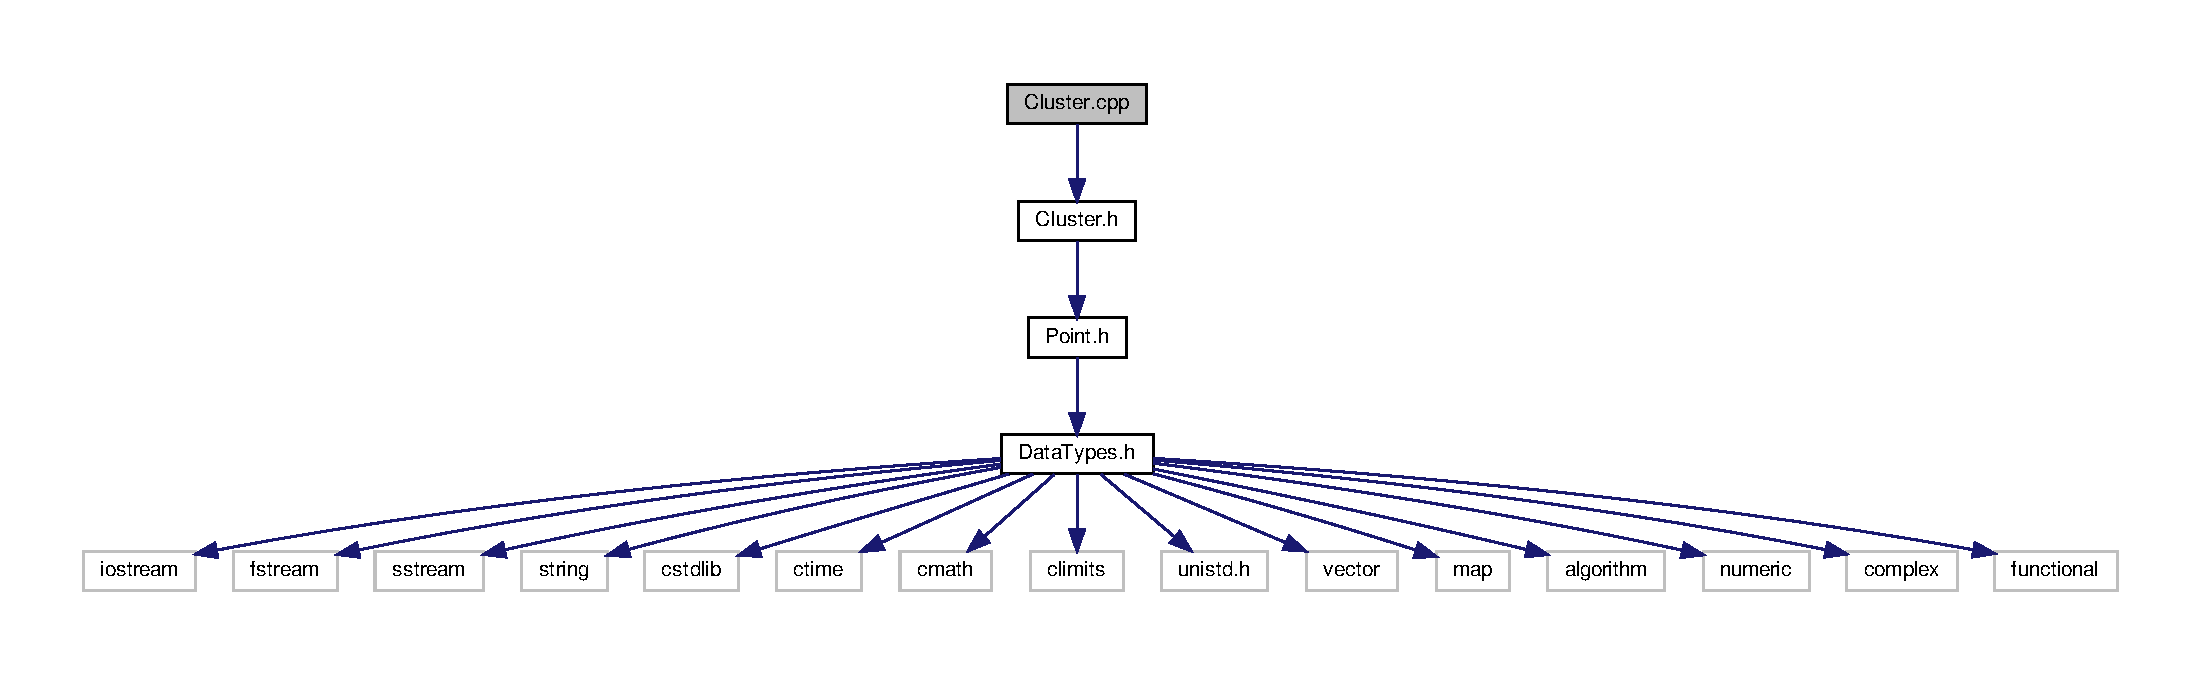
\includegraphics[width=350pt]{_cluster_8cpp__incl}
\end{center}
\end{figure}

\section{Cluster.\+h File Reference}
\label{_cluster_8h}\index{Cluster.\+h@{Cluster.\+h}}
{\ttfamily \#include \char`\"{}Point.\+h\char`\"{}}\newline
Include dependency graph for Cluster.\+h\+:\nopagebreak
\begin{figure}[H]
\begin{center}
\leavevmode
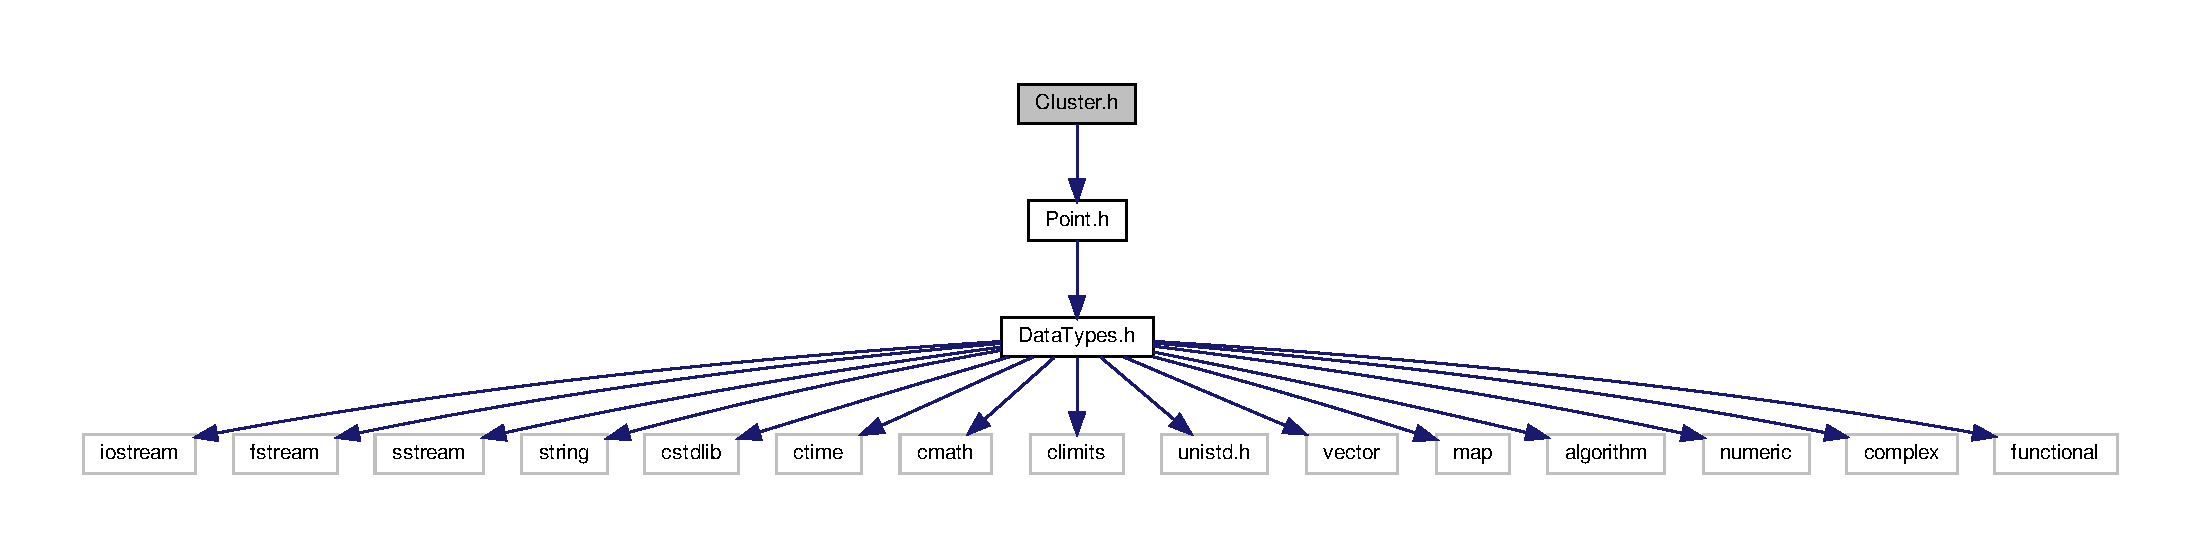
\includegraphics[width=350pt]{_cluster_8h__incl}
\end{center}
\end{figure}
This graph shows which files directly or indirectly include this file\+:\nopagebreak
\begin{figure}[H]
\begin{center}
\leavevmode
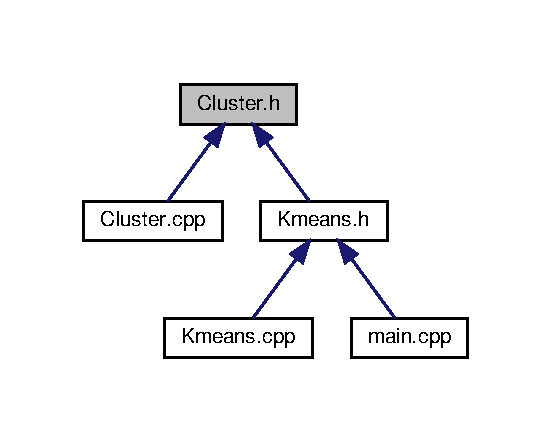
\includegraphics[width=265pt]{_cluster_8h__dep__incl}
\end{center}
\end{figure}
\subsection*{Classes}
\begin{DoxyCompactItemize}
\item 
class \textbf{ Cluster}
\end{DoxyCompactItemize}

\section{Data\+Types.\+h File Reference}
\label{_data_types_8h}\index{Data\+Types.\+h@{Data\+Types.\+h}}
{\ttfamily \#include $<$iostream$>$}\newline
{\ttfamily \#include $<$fstream$>$}\newline
{\ttfamily \#include $<$sstream$>$}\newline
{\ttfamily \#include $<$string$>$}\newline
{\ttfamily \#include $<$cstdlib$>$}\newline
{\ttfamily \#include $<$ctime$>$}\newline
{\ttfamily \#include $<$cmath$>$}\newline
{\ttfamily \#include $<$climits$>$}\newline
{\ttfamily \#include $<$unistd.\+h$>$}\newline
{\ttfamily \#include $<$vector$>$}\newline
{\ttfamily \#include $<$map$>$}\newline
{\ttfamily \#include $<$algorithm$>$}\newline
{\ttfamily \#include $<$numeric$>$}\newline
{\ttfamily \#include $<$complex$>$}\newline
{\ttfamily \#include $<$functional$>$}\newline
Include dependency graph for Data\+Types.\+h\+:
\nopagebreak
\begin{figure}[H]
\begin{center}
\leavevmode
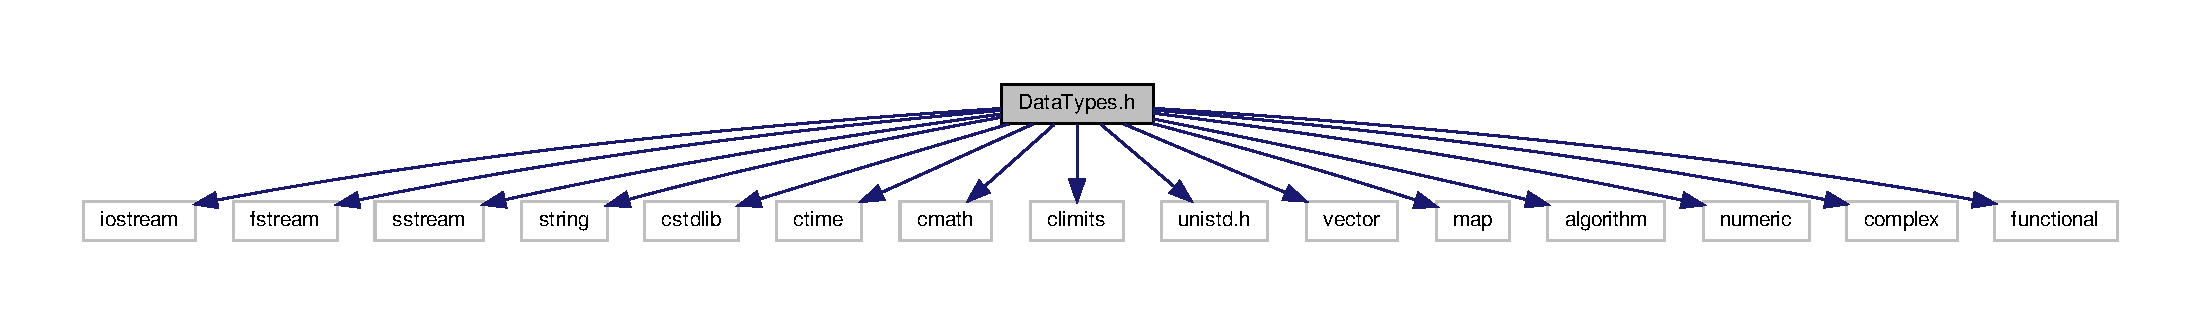
\includegraphics[width=350pt]{_data_types_8h__incl}
\end{center}
\end{figure}
This graph shows which files directly or indirectly include this file\+:
\nopagebreak
\begin{figure}[H]
\begin{center}
\leavevmode
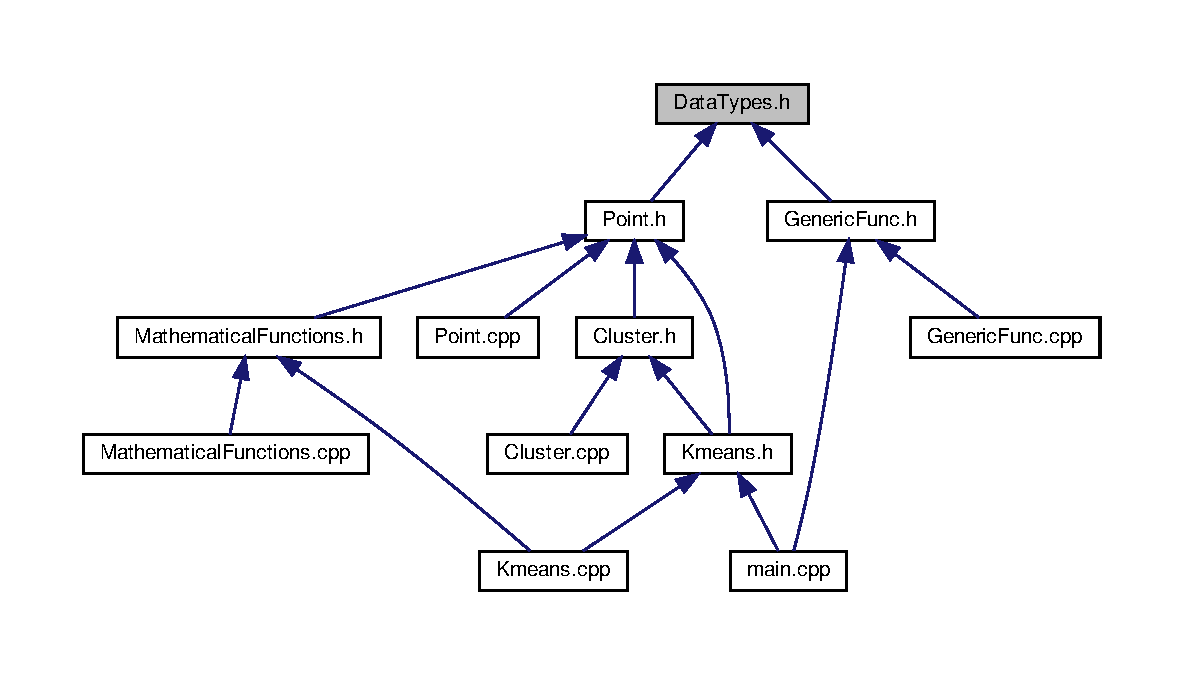
\includegraphics[width=350pt]{_data_types_8h__dep__incl}
\end{center}
\end{figure}
\subsection*{Typedefs}
\begin{DoxyCompactItemize}
\item 
typedef std\+::vector$<$ float $>$ \textbf{ Float\+Vector}
\item 
typedef std\+::vector$<$ \textbf{ Float\+Vector} $>$ \textbf{ Float\+Vector2D}
\item 
typedef std\+::vector$<$ double $>$ \textbf{ Double\+Vector}
\item 
typedef std\+::vector$<$ \textbf{ Double\+Vector} $>$ \textbf{ Double\+Vector2D}
\item 
typedef std\+::vector$<$ int $>$ \textbf{ Int\+Vector}
\item 
typedef std\+::vector$<$ \textbf{ Int\+Vector} $>$ \textbf{ Int\+Vector2D}
\item 
typedef std\+::vector$<$ std\+::string $>$ \textbf{ String\+Vector}
\item 
typedef std\+::vector$<$ \textbf{ String\+Vector} $>$ \textbf{ String\+Vector2D}
\item 
typedef std\+::pair$<$ int, int $>$ \textbf{ Int\+Int\+Pair}
\item 
typedef std\+::pair$<$ int, float $>$ \textbf{ Int\+Float\+Pair}
\item 
typedef std\+::map$<$ int, int $>$ \textbf{ Int\+Int\+Map}
\item 
typedef std\+::map$<$ int, \textbf{ Int\+Vector} $>$ \textbf{ Int\+Int\+Vector\+Map}
\item 
typedef std\+::map$<$ int, \textbf{ Float\+Vector} $>$ \textbf{ Int\+Float\+Vector\+Map}
\end{DoxyCompactItemize}


\subsection{Typedef Documentation}
\mbox{\label{_data_types_8h_a82f6bc76e1c7a0f51bf3e95ad5d3c590}} 
\index{Data\+Types.\+h@{Data\+Types.\+h}!Double\+Vector@{Double\+Vector}}
\index{Double\+Vector@{Double\+Vector}!Data\+Types.\+h@{Data\+Types.\+h}}
\subsubsection{Double\+Vector}
{\footnotesize\ttfamily typedef std\+::vector$<$double$>$ \textbf{ Double\+Vector}}



Definition at line 25 of file Data\+Types.\+h.

\mbox{\label{_data_types_8h_a7e70d37182fdafec492c4dd396c9698c}} 
\index{Data\+Types.\+h@{Data\+Types.\+h}!Double\+Vector2D@{Double\+Vector2D}}
\index{Double\+Vector2D@{Double\+Vector2D}!Data\+Types.\+h@{Data\+Types.\+h}}
\subsubsection{Double\+Vector2D}
{\footnotesize\ttfamily typedef std\+::vector$<$\textbf{ Double\+Vector}$>$ \textbf{ Double\+Vector2D}}



Definition at line 26 of file Data\+Types.\+h.

\mbox{\label{_data_types_8h_a64be07a13efb96ba9d376c4cbc6f501e}} 
\index{Data\+Types.\+h@{Data\+Types.\+h}!Float\+Vector@{Float\+Vector}}
\index{Float\+Vector@{Float\+Vector}!Data\+Types.\+h@{Data\+Types.\+h}}
\subsubsection{Float\+Vector}
{\footnotesize\ttfamily typedef std\+::vector$<$float$>$ \textbf{ Float\+Vector}}



Definition at line 23 of file Data\+Types.\+h.

\mbox{\label{_data_types_8h_a90fed7f97f1803c7719d26e6f21b4de6}} 
\index{Data\+Types.\+h@{Data\+Types.\+h}!Float\+Vector2D@{Float\+Vector2D}}
\index{Float\+Vector2D@{Float\+Vector2D}!Data\+Types.\+h@{Data\+Types.\+h}}
\subsubsection{Float\+Vector2D}
{\footnotesize\ttfamily typedef std\+::vector$<$\textbf{ Float\+Vector}$>$ \textbf{ Float\+Vector2D}}



Definition at line 24 of file Data\+Types.\+h.

\mbox{\label{_data_types_8h_a3d5049745a50e0c457cb380125e045dc}} 
\index{Data\+Types.\+h@{Data\+Types.\+h}!Int\+Float\+Pair@{Int\+Float\+Pair}}
\index{Int\+Float\+Pair@{Int\+Float\+Pair}!Data\+Types.\+h@{Data\+Types.\+h}}
\subsubsection{Int\+Float\+Pair}
{\footnotesize\ttfamily typedef std\+::pair$<$int,float$>$ \textbf{ Int\+Float\+Pair}}



Definition at line 32 of file Data\+Types.\+h.

\mbox{\label{_data_types_8h_ae9ec0f616e5edddb88bd7cba63e2ea88}} 
\index{Data\+Types.\+h@{Data\+Types.\+h}!Int\+Float\+Vector\+Map@{Int\+Float\+Vector\+Map}}
\index{Int\+Float\+Vector\+Map@{Int\+Float\+Vector\+Map}!Data\+Types.\+h@{Data\+Types.\+h}}
\subsubsection{Int\+Float\+Vector\+Map}
{\footnotesize\ttfamily typedef std\+::map$<$int,\textbf{ Float\+Vector}$>$ \textbf{ Int\+Float\+Vector\+Map}}



Definition at line 35 of file Data\+Types.\+h.

\mbox{\label{_data_types_8h_a1972afbb2da11833cc5c4e7dda7936cf}} 
\index{Data\+Types.\+h@{Data\+Types.\+h}!Int\+Int\+Map@{Int\+Int\+Map}}
\index{Int\+Int\+Map@{Int\+Int\+Map}!Data\+Types.\+h@{Data\+Types.\+h}}
\subsubsection{Int\+Int\+Map}
{\footnotesize\ttfamily typedef std\+::map$<$int,int$>$ \textbf{ Int\+Int\+Map}}



Definition at line 33 of file Data\+Types.\+h.

\mbox{\label{_data_types_8h_aafe152bbcb51930b658b8a4406f4d67e}} 
\index{Data\+Types.\+h@{Data\+Types.\+h}!Int\+Int\+Pair@{Int\+Int\+Pair}}
\index{Int\+Int\+Pair@{Int\+Int\+Pair}!Data\+Types.\+h@{Data\+Types.\+h}}
\subsubsection{Int\+Int\+Pair}
{\footnotesize\ttfamily typedef std\+::pair$<$int,int$>$ \textbf{ Int\+Int\+Pair}}



Definition at line 31 of file Data\+Types.\+h.

\mbox{\label{_data_types_8h_afae9076c89b4ed1654b0f85beb47af82}} 
\index{Data\+Types.\+h@{Data\+Types.\+h}!Int\+Int\+Vector\+Map@{Int\+Int\+Vector\+Map}}
\index{Int\+Int\+Vector\+Map@{Int\+Int\+Vector\+Map}!Data\+Types.\+h@{Data\+Types.\+h}}
\subsubsection{Int\+Int\+Vector\+Map}
{\footnotesize\ttfamily typedef std\+::map$<$int,\textbf{ Int\+Vector}$>$ \textbf{ Int\+Int\+Vector\+Map}}



Definition at line 34 of file Data\+Types.\+h.

\mbox{\label{_data_types_8h_a9b8f2f96749808efd0d975e75d96a71c}} 
\index{Data\+Types.\+h@{Data\+Types.\+h}!Int\+Vector@{Int\+Vector}}
\index{Int\+Vector@{Int\+Vector}!Data\+Types.\+h@{Data\+Types.\+h}}
\subsubsection{Int\+Vector}
{\footnotesize\ttfamily typedef std\+::vector$<$int$>$ \textbf{ Int\+Vector}}



Definition at line 27 of file Data\+Types.\+h.

\mbox{\label{_data_types_8h_a2611314ab2c7ffc99f4b34f959b4723c}} 
\index{Data\+Types.\+h@{Data\+Types.\+h}!Int\+Vector2D@{Int\+Vector2D}}
\index{Int\+Vector2D@{Int\+Vector2D}!Data\+Types.\+h@{Data\+Types.\+h}}
\subsubsection{Int\+Vector2D}
{\footnotesize\ttfamily typedef std\+::vector$<$\textbf{ Int\+Vector}$>$ \textbf{ Int\+Vector2D}}



Definition at line 28 of file Data\+Types.\+h.

\mbox{\label{_data_types_8h_ab8e1ede88e2ff1c3b448334e6cbd3533}} 
\index{Data\+Types.\+h@{Data\+Types.\+h}!String\+Vector@{String\+Vector}}
\index{String\+Vector@{String\+Vector}!Data\+Types.\+h@{Data\+Types.\+h}}
\subsubsection{String\+Vector}
{\footnotesize\ttfamily typedef std\+::vector$<$std\+::string$>$ \textbf{ String\+Vector}}



Definition at line 29 of file Data\+Types.\+h.

\mbox{\label{_data_types_8h_acccc44108a5c4da23723c861fdaf8ed5}} 
\index{Data\+Types.\+h@{Data\+Types.\+h}!String\+Vector2D@{String\+Vector2D}}
\index{String\+Vector2D@{String\+Vector2D}!Data\+Types.\+h@{Data\+Types.\+h}}
\subsubsection{String\+Vector2D}
{\footnotesize\ttfamily typedef std\+::vector$<$\textbf{ String\+Vector}$>$ \textbf{ String\+Vector2D}}



Definition at line 30 of file Data\+Types.\+h.


\section{File\+Func.\+h File Reference}
\label{_file_func_8h}\index{File\+Func.\+h@{File\+Func.\+h}}
{\ttfamily \#include $<$vector$>$}\newline
Include dependency graph for File\+Func.\+h\+:\nopagebreak
\begin{figure}[H]
\begin{center}
\leavevmode
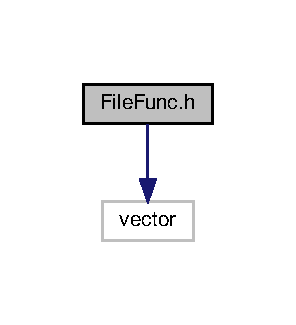
\includegraphics[width=142pt]{_file_func_8h__incl}
\end{center}
\end{figure}
\subsection*{Namespaces}
\begin{DoxyCompactItemize}
\item 
 \textbf{ flnc}
\end{DoxyCompactItemize}
\subsection*{Typedefs}
\begin{DoxyCompactItemize}
\item 
typedef std\+::basic\+\_\+istream$<$ char, std\+::char\+\_\+traits$<$ char $>$ $>$ \textbf{ minput\+\_\+stream}
\item 
typedef std\+::basic\+\_\+ostream$<$ char, std\+::char\+\_\+traits$<$ char $>$ $>$ \textbf{ moutput\+\_\+stream}
\end{DoxyCompactItemize}
\subsection*{Functions}
\begin{DoxyCompactItemize}
\item 
{\footnotesize template$<$typename T\+Y\+PE $>$ }\\void \textbf{ flnc\+::\+Write\+Vector\+To\+File} (\textbf{ moutput\+\_\+stream} $\ast$Training\+File\+Out, const std\+::vector$<$ T\+Y\+PE $>$ \&vec)
\item 
{\footnotesize template$<$typename T\+Y\+PE $>$ }\\void \textbf{ flnc\+::\+Write2\+D\+Vector\+To\+File} (\textbf{ moutput\+\_\+stream} $\ast$Training\+File\+Out, const std\+::vector$<$ std\+::vector$<$ T\+Y\+PE $>$ $>$ \&vec)
\item 
{\footnotesize template$<$typename T\+Y\+PE $>$ }\\void \textbf{ flnc\+::\+Read\+Vector\+From\+File} (\textbf{ minput\+\_\+stream} $\ast$Training\+File\+In, std\+::vector$<$ T\+Y\+PE $>$ \&vec)
\item 
{\footnotesize template$<$typename T\+Y\+PE $>$ }\\void \textbf{ flnc\+::\+Read2\+D\+Vector\+From\+File} (\textbf{ minput\+\_\+stream} $\ast$Training\+File\+In, std\+::vector$<$ std\+::vector$<$ T\+Y\+PE $>$ $>$ \&vec)
\end{DoxyCompactItemize}


\subsection{Typedef Documentation}
\mbox{\label{_file_func_8h_ac7d0feb122d3a455f1a91ba26b3de612}} 
\index{File\+Func.\+h@{File\+Func.\+h}!minput\+\_\+stream@{minput\+\_\+stream}}
\index{minput\+\_\+stream@{minput\+\_\+stream}!File\+Func.\+h@{File\+Func.\+h}}
\subsubsection{minput\+\_\+stream}
{\footnotesize\ttfamily typedef std\+::basic\+\_\+istream$<$char,std\+::char\+\_\+traits$<$char$>$ $>$ \textbf{ minput\+\_\+stream}}



Definition at line 5 of file File\+Func.\+h.

\mbox{\label{_file_func_8h_adf5ef842b05a918896d7eb7755bbee56}} 
\index{File\+Func.\+h@{File\+Func.\+h}!moutput\+\_\+stream@{moutput\+\_\+stream}}
\index{moutput\+\_\+stream@{moutput\+\_\+stream}!File\+Func.\+h@{File\+Func.\+h}}
\subsubsection{moutput\+\_\+stream}
{\footnotesize\ttfamily typedef std\+::basic\+\_\+ostream$<$char,std\+::char\+\_\+traits$<$char$>$ $>$ \textbf{ moutput\+\_\+stream}}



Definition at line 6 of file File\+Func.\+h.


\section{Generic\+Func.\+cpp File Reference}
\label{_generic_func_8cpp}\index{Generic\+Func.\+cpp@{Generic\+Func.\+cpp}}
{\ttfamily \#include \char`\"{}Generic\+Func.\+h\char`\"{}}\newline
Include dependency graph for Generic\+Func.\+cpp\+:\nopagebreak
\begin{figure}[H]
\begin{center}
\leavevmode
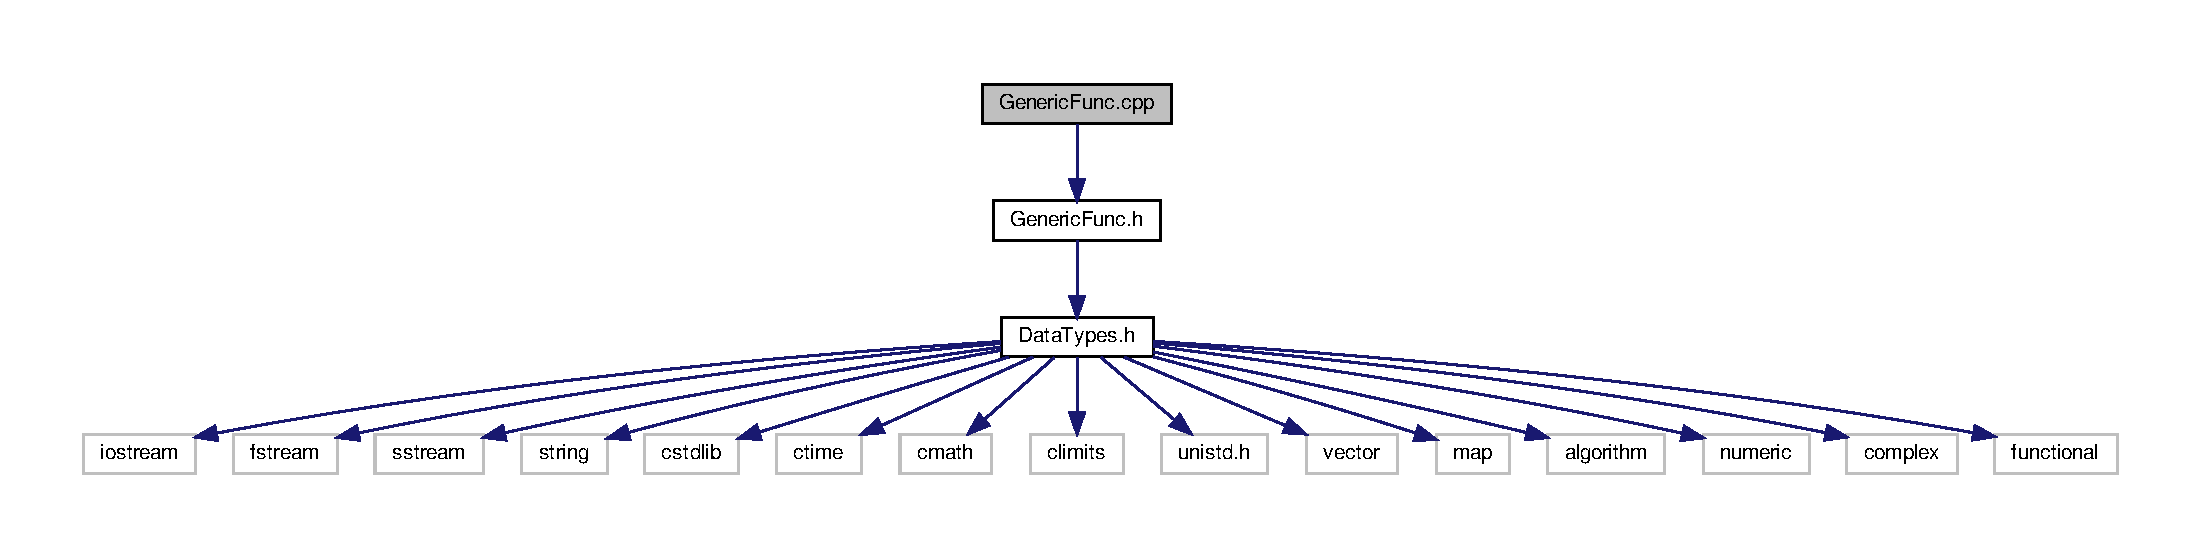
\includegraphics[width=350pt]{_generic_func_8cpp__incl}
\end{center}
\end{figure}

\section{Generic\+Func.\+h File Reference}
\label{_generic_func_8h}\index{Generic\+Func.\+h@{Generic\+Func.\+h}}
{\ttfamily \#include \char`\"{}Data\+Types.\+h\char`\"{}}\newline
Include dependency graph for Generic\+Func.\+h\+:
\nopagebreak
\begin{figure}[H]
\begin{center}
\leavevmode
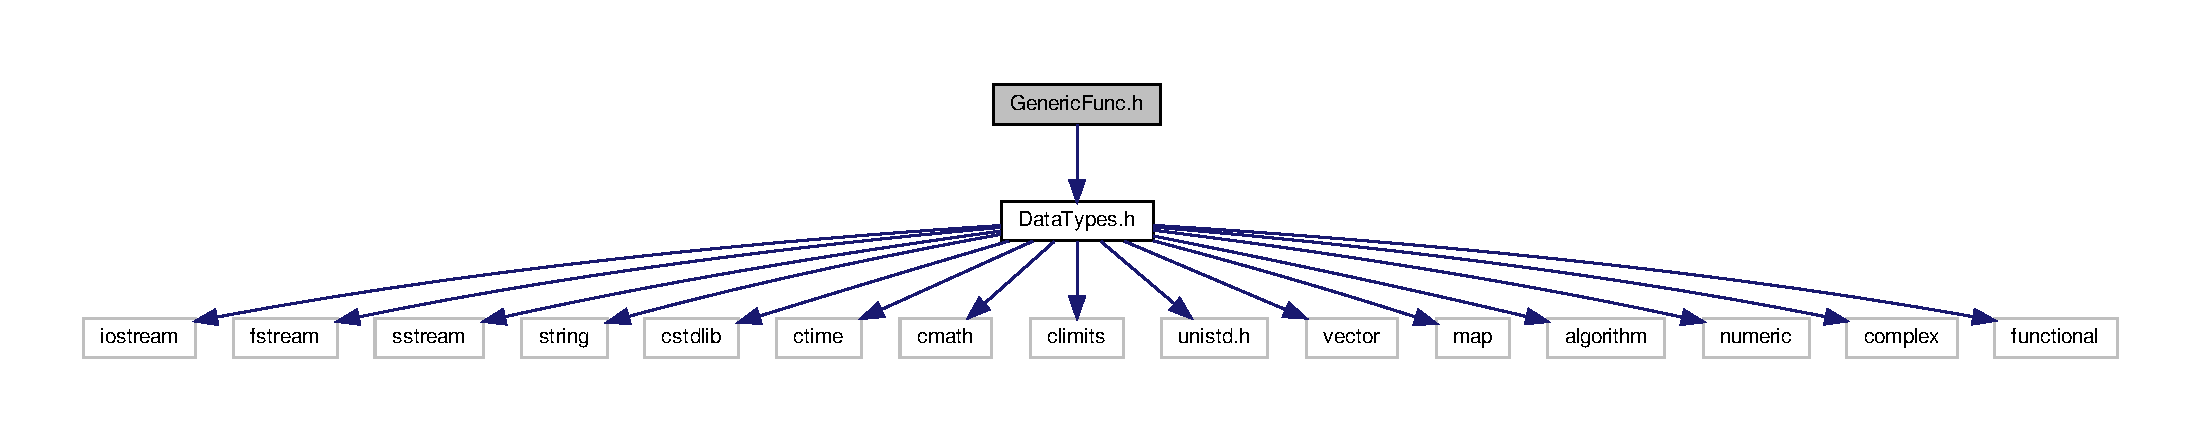
\includegraphics[width=350pt]{_generic_func_8h__incl}
\end{center}
\end{figure}
This graph shows which files directly or indirectly include this file\+:
\nopagebreak
\begin{figure}[H]
\begin{center}
\leavevmode
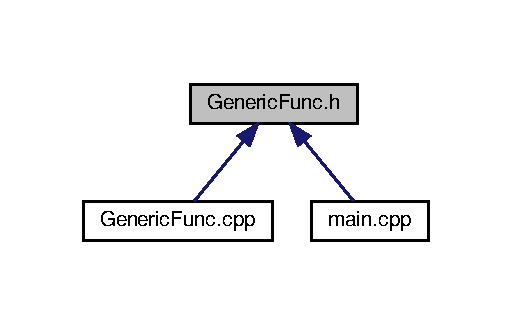
\includegraphics[width=246pt]{_generic_func_8h__dep__incl}
\end{center}
\end{figure}
\subsection*{Namespaces}
\begin{DoxyCompactItemize}
\item 
 \textbf{ gf}
\end{DoxyCompactItemize}
\subsection*{Functions}
\begin{DoxyCompactItemize}
\item 
std\+::string \textbf{ gf\+::get\+Executable\+Path} ()
\item 
std\+::string \textbf{ gf\+::get\+Executable\+Path\+And\+Match\+It\+With\+Filename} (std\+::string filename)
\end{DoxyCompactItemize}

\section{Kmeans.\+cpp File Reference}
\label{_kmeans_8cpp}\index{Kmeans.\+cpp@{Kmeans.\+cpp}}
{\ttfamily \#include \char`\"{}Kmeans.\+h\char`\"{}}\newline
{\ttfamily \#include \char`\"{}Properties\+Parser.\+h\char`\"{}}\newline
{\ttfamily \#include \char`\"{}Mathematical\+Functions.\+h\char`\"{}}\newline
Include dependency graph for Kmeans.\+cpp\+:\nopagebreak
\begin{figure}[H]
\begin{center}
\leavevmode
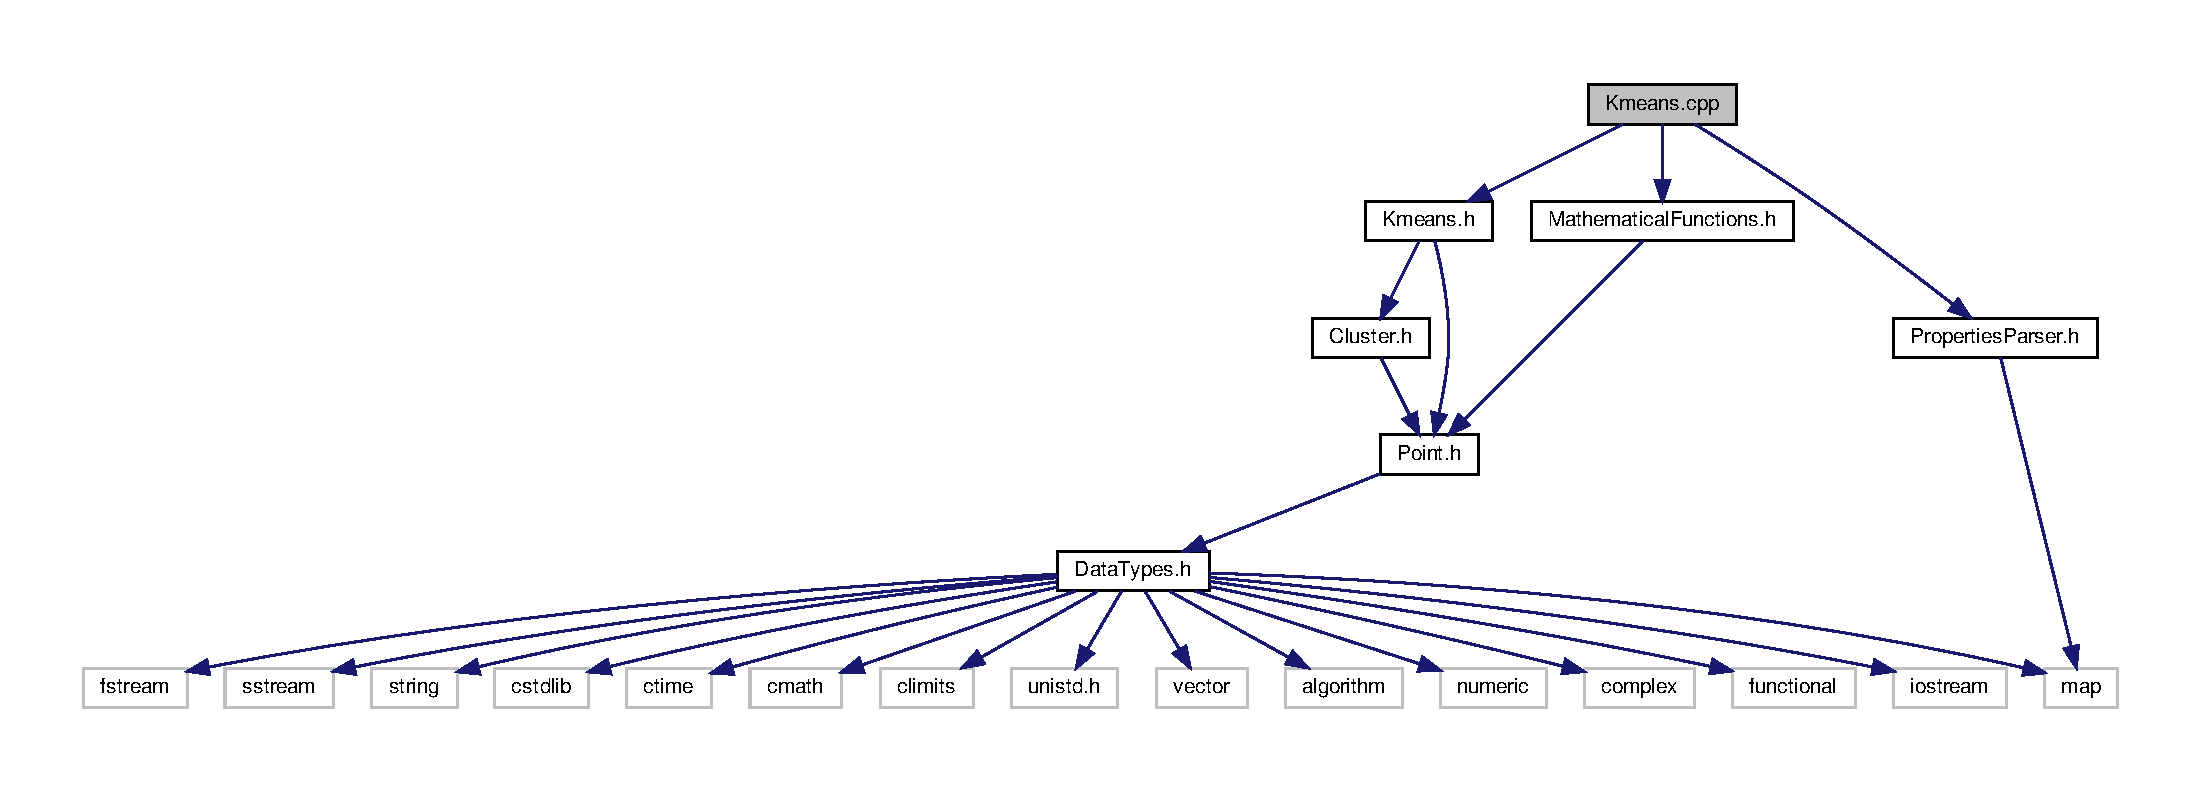
\includegraphics[width=350pt]{_kmeans_8cpp__incl}
\end{center}
\end{figure}
\subsection*{Functions}
\begin{DoxyCompactItemize}
\item 
bool \textbf{ less\+\_\+f} (const \textbf{ Int\+Int\+Pair} \&pair\+\_\+a, const \textbf{ Int\+Int\+Pair} \&pair\+\_\+b)
\end{DoxyCompactItemize}


\subsection{Function Documentation}
\mbox{\label{_kmeans_8cpp_af55f0370ee6815bfd82fce81e16ad74e}} 
\index{Kmeans.\+cpp@{Kmeans.\+cpp}!less\+\_\+f@{less\+\_\+f}}
\index{less\+\_\+f@{less\+\_\+f}!Kmeans.\+cpp@{Kmeans.\+cpp}}
\subsubsection{less\+\_\+f()}
{\footnotesize\ttfamily bool less\+\_\+f (\begin{DoxyParamCaption}\item[{const \textbf{ Int\+Int\+Pair} \&}]{pair\+\_\+a,  }\item[{const \textbf{ Int\+Int\+Pair} \&}]{pair\+\_\+b }\end{DoxyParamCaption})}



Definition at line 5 of file Kmeans.\+cpp.


\section{Kmeans.\+h File Reference}
\label{_kmeans_8h}\index{Kmeans.\+h@{Kmeans.\+h}}
{\ttfamily \#include \char`\"{}Point.\+h\char`\"{}}\newline
{\ttfamily \#include \char`\"{}Cluster.\+h\char`\"{}}\newline
Include dependency graph for Kmeans.\+h\+:
\nopagebreak
\begin{figure}[H]
\begin{center}
\leavevmode
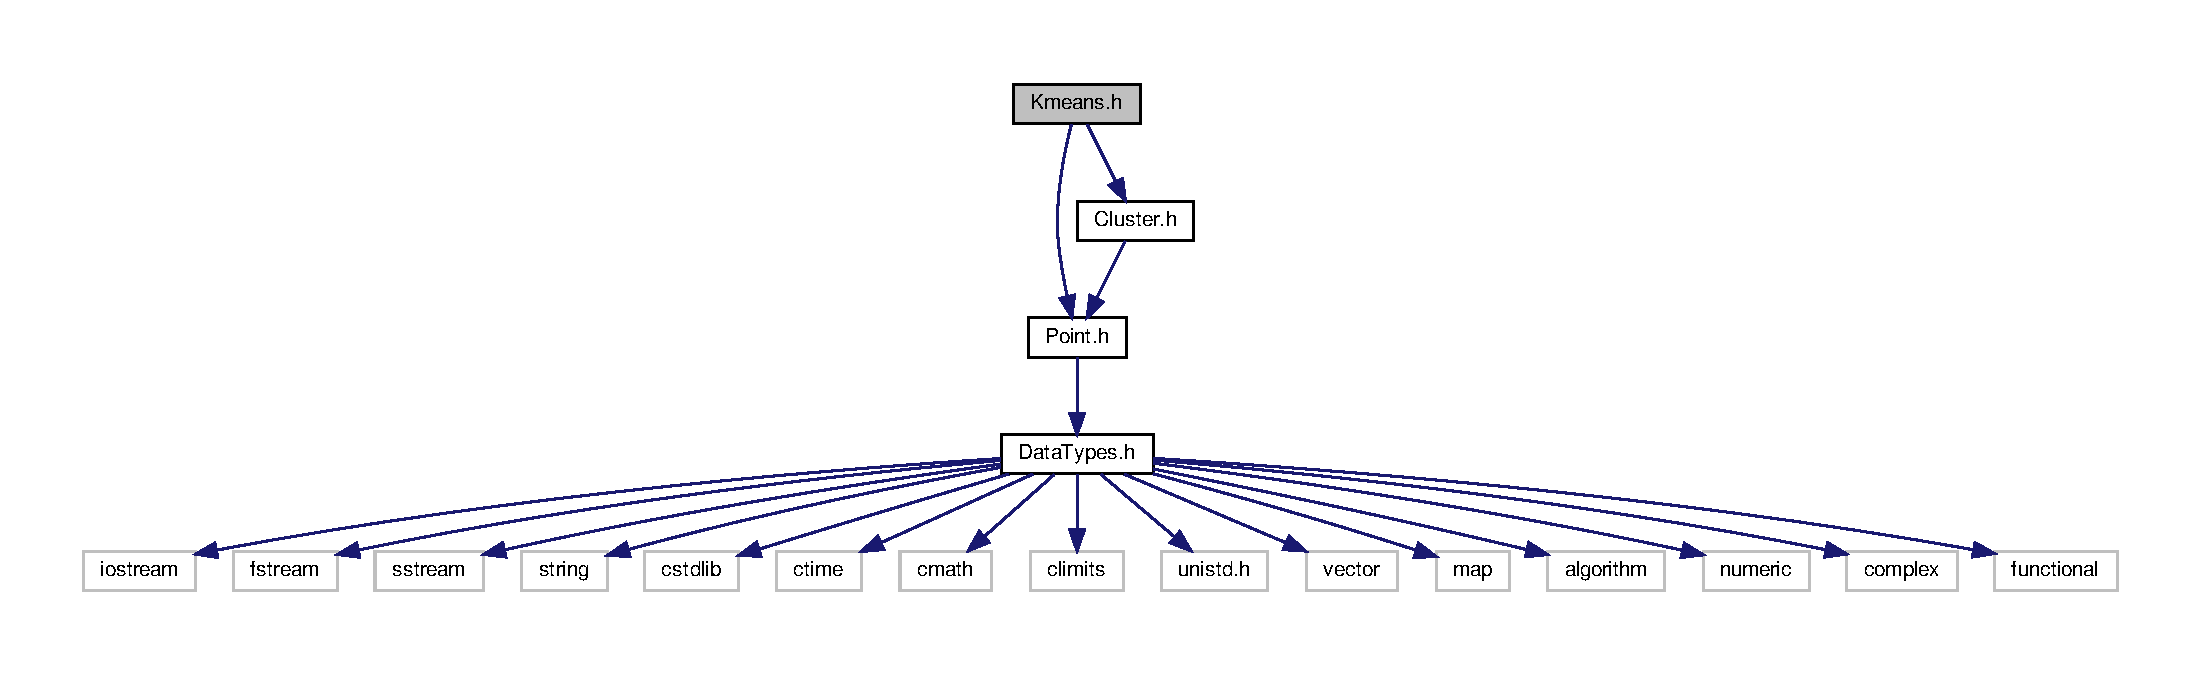
\includegraphics[width=350pt]{_kmeans_8h__incl}
\end{center}
\end{figure}
This graph shows which files directly or indirectly include this file\+:
\nopagebreak
\begin{figure}[H]
\begin{center}
\leavevmode
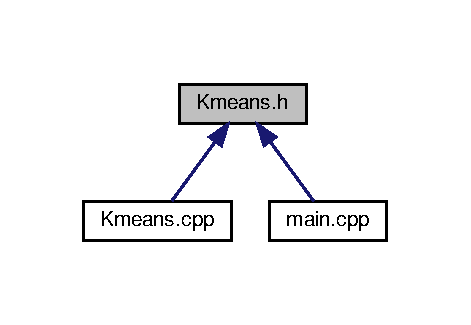
\includegraphics[width=226pt]{_kmeans_8h__dep__incl}
\end{center}
\end{figure}
\subsection*{Classes}
\begin{DoxyCompactItemize}
\item 
class \textbf{ Kmeans}
\end{DoxyCompactItemize}

\section{main.\+cpp File Reference}
\label{main_8cpp}\index{main.\+cpp@{main.\+cpp}}
{\ttfamily \#include \char`\"{}Kmeans.\+h\char`\"{}}\newline
{\ttfamily \#include \char`\"{}Generic\+Func.\+h\char`\"{}}\newline
Include dependency graph for main.\+cpp\+:\nopagebreak
\begin{figure}[H]
\begin{center}
\leavevmode
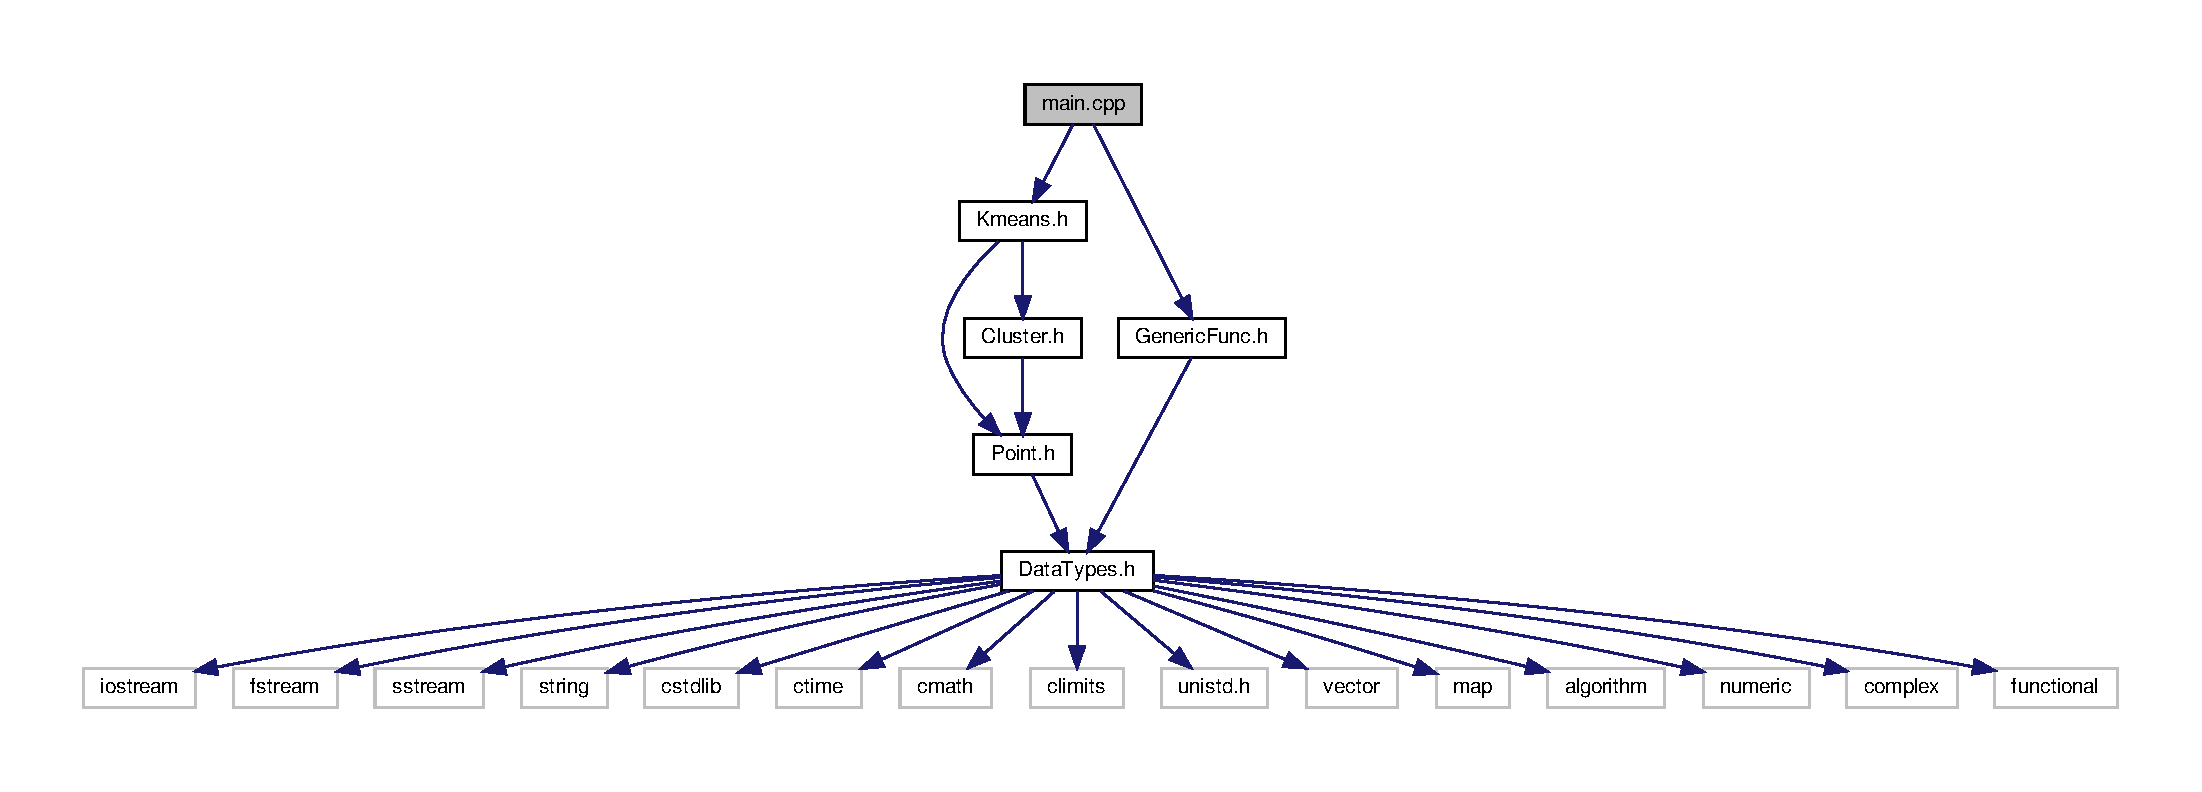
\includegraphics[width=350pt]{main_8cpp__incl}
\end{center}
\end{figure}
\subsection*{Functions}
\begin{DoxyCompactItemize}
\item 
int \textbf{ main} ()
\end{DoxyCompactItemize}


\subsection{Function Documentation}
\mbox{\label{main_8cpp_ae66f6b31b5ad750f1fe042a706a4e3d4}} 
\index{main.\+cpp@{main.\+cpp}!main@{main}}
\index{main@{main}!main.\+cpp@{main.\+cpp}}
\subsubsection{main()}
{\footnotesize\ttfamily int main (\begin{DoxyParamCaption}{ }\end{DoxyParamCaption})}



Definition at line 4 of file main.\+cpp.


\section{Mathematical\+Functions.\+cpp File Reference}
\label{_mathematical_functions_8cpp}\index{Mathematical\+Functions.\+cpp@{Mathematical\+Functions.\+cpp}}
{\ttfamily \#include \char`\"{}Mathematical\+Functions.\+h\char`\"{}}\newline
Include dependency graph for Mathematical\+Functions.\+cpp\+:\nopagebreak
\begin{figure}[H]
\begin{center}
\leavevmode
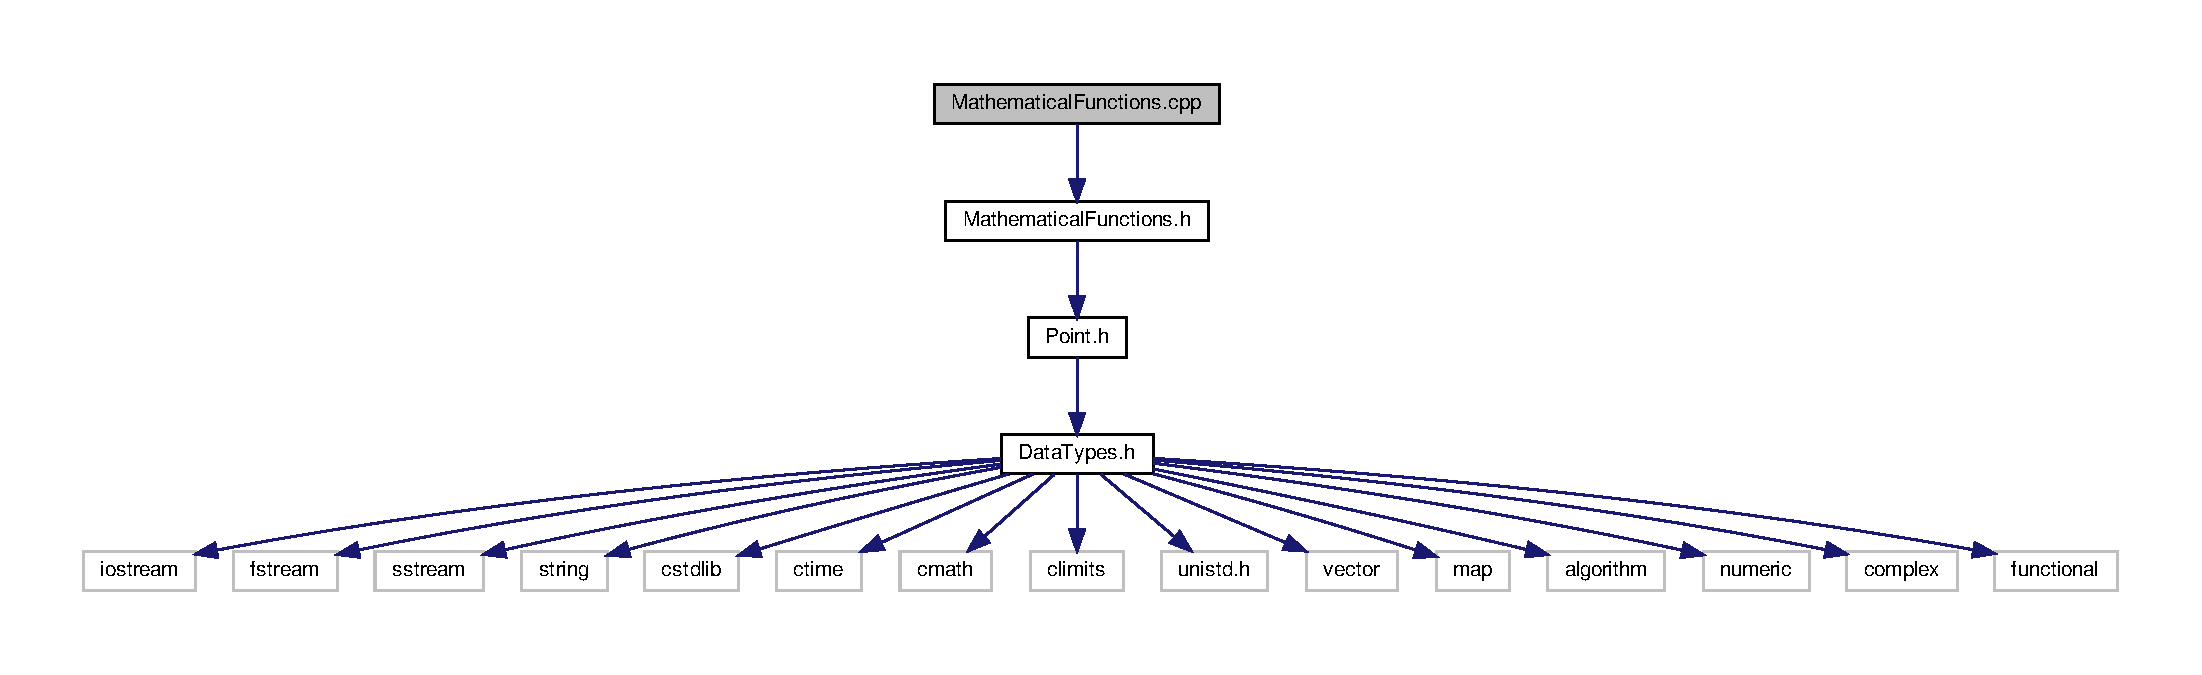
\includegraphics[width=350pt]{_mathematical_functions_8cpp__incl}
\end{center}
\end{figure}

\section{Mathematical\+Functions.\+h File Reference}
\label{_mathematical_functions_8h}\index{Mathematical\+Functions.\+h@{Mathematical\+Functions.\+h}}
{\ttfamily \#include \char`\"{}Point.\+h\char`\"{}}\newline
Include dependency graph for Mathematical\+Functions.\+h\+:\nopagebreak
\begin{figure}[H]
\begin{center}
\leavevmode
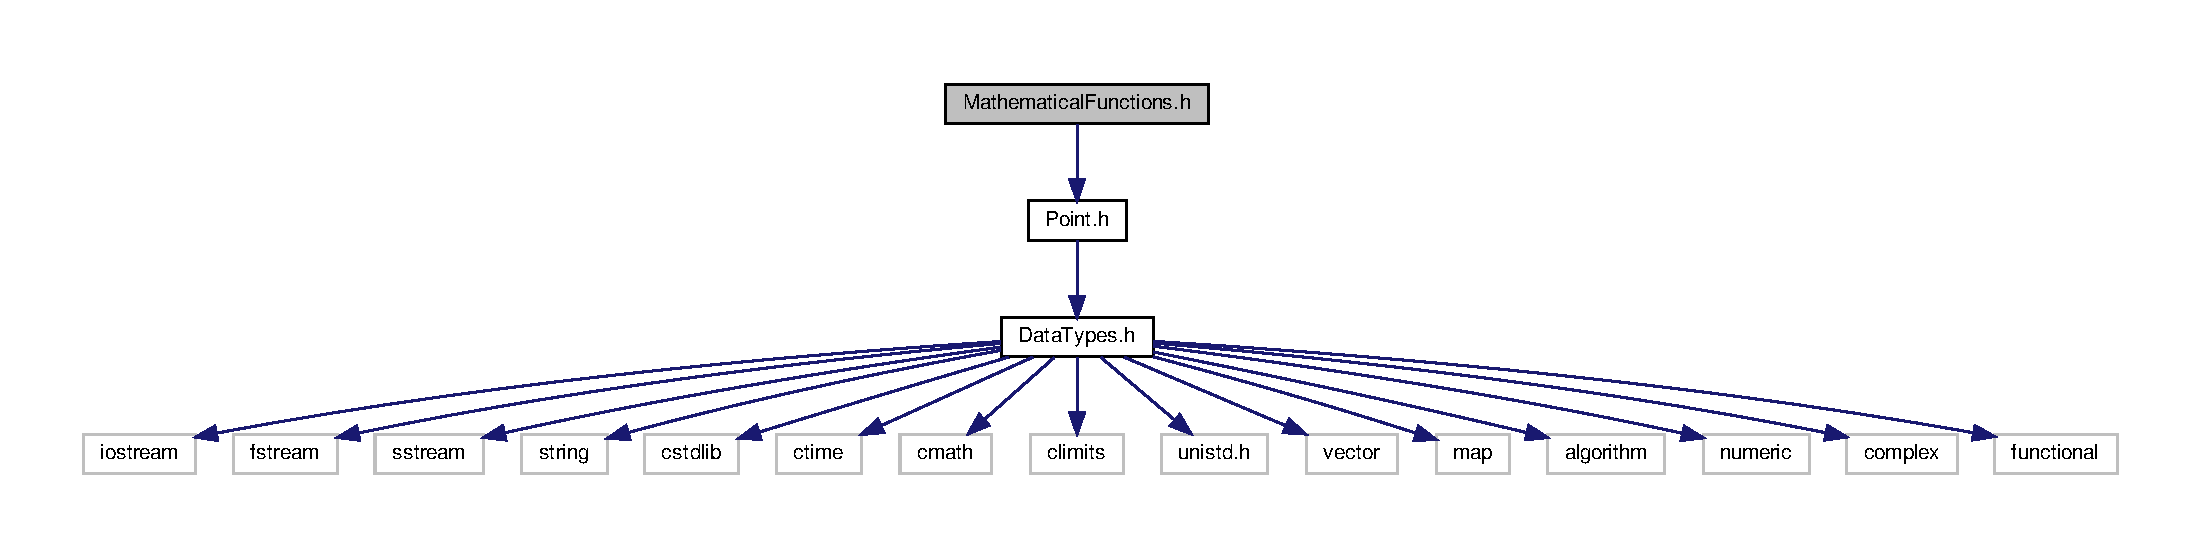
\includegraphics[width=350pt]{_mathematical_functions_8h__incl}
\end{center}
\end{figure}
This graph shows which files directly or indirectly include this file\+:\nopagebreak
\begin{figure}[H]
\begin{center}
\leavevmode
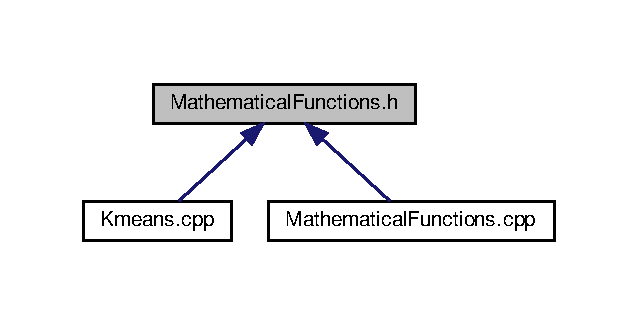
\includegraphics[width=306pt]{_mathematical_functions_8h__dep__incl}
\end{center}
\end{figure}
\subsection*{Namespaces}
\begin{DoxyCompactItemize}
\item 
 \textbf{ mf}
\end{DoxyCompactItemize}
\subsection*{Functions}
\begin{DoxyCompactItemize}
\item 
size\+\_\+t \textbf{ mf\+::min\+Size} (\textbf{ Point} \&p, \textbf{ Point} \&q)
\item 
double \textbf{ mf\+::mean} (\textbf{ Point} \&p)
\item 
double \textbf{ mf\+::st\+Dev} (\textbf{ Point} \&p)
\item 
double \textbf{ mf\+::euclidean\+Distance} (\textbf{ Point} \&p, \textbf{ Point} \&q)
\item 
double \textbf{ mf\+::euclidean\+Distance\+Squared} (\textbf{ Point} \&p, \textbf{ Point} \&q)
\item 
double \textbf{ mf\+::manhattan\+Distance} (\textbf{ Point} \&p, \textbf{ Point} \&q)
\item 
double \textbf{ mf\+::chebyshev\+Distance} (\textbf{ Point} \&p, \textbf{ Point} \&q)
\item 
double \textbf{ mf\+::bray\+Curtis\+Distance} (\textbf{ Point} \&p, \textbf{ Point} \&q)
\item 
double \textbf{ mf\+::canberra\+Distance} (\textbf{ Point} \&p, \textbf{ Point} \&q)
\item 
double \textbf{ mf\+::pearson\+Correlation} (\textbf{ Point} \&p, \textbf{ Point} \&q)
\item 
double \textbf{ mf\+::cosine\+Similarity} (\textbf{ Point} \&p, \textbf{ Point} \&q)
\item 
double \textbf{ mf\+::dot} (\textbf{ Point} \&p, \textbf{ Point} \&q)
\end{DoxyCompactItemize}

\section{Point.\+cpp File Reference}
\label{_point_8cpp}\index{Point.\+cpp@{Point.\+cpp}}
{\ttfamily \#include \char`\"{}Point.\+h\char`\"{}}\newline
Include dependency graph for Point.\+cpp\+:\nopagebreak
\begin{figure}[H]
\begin{center}
\leavevmode
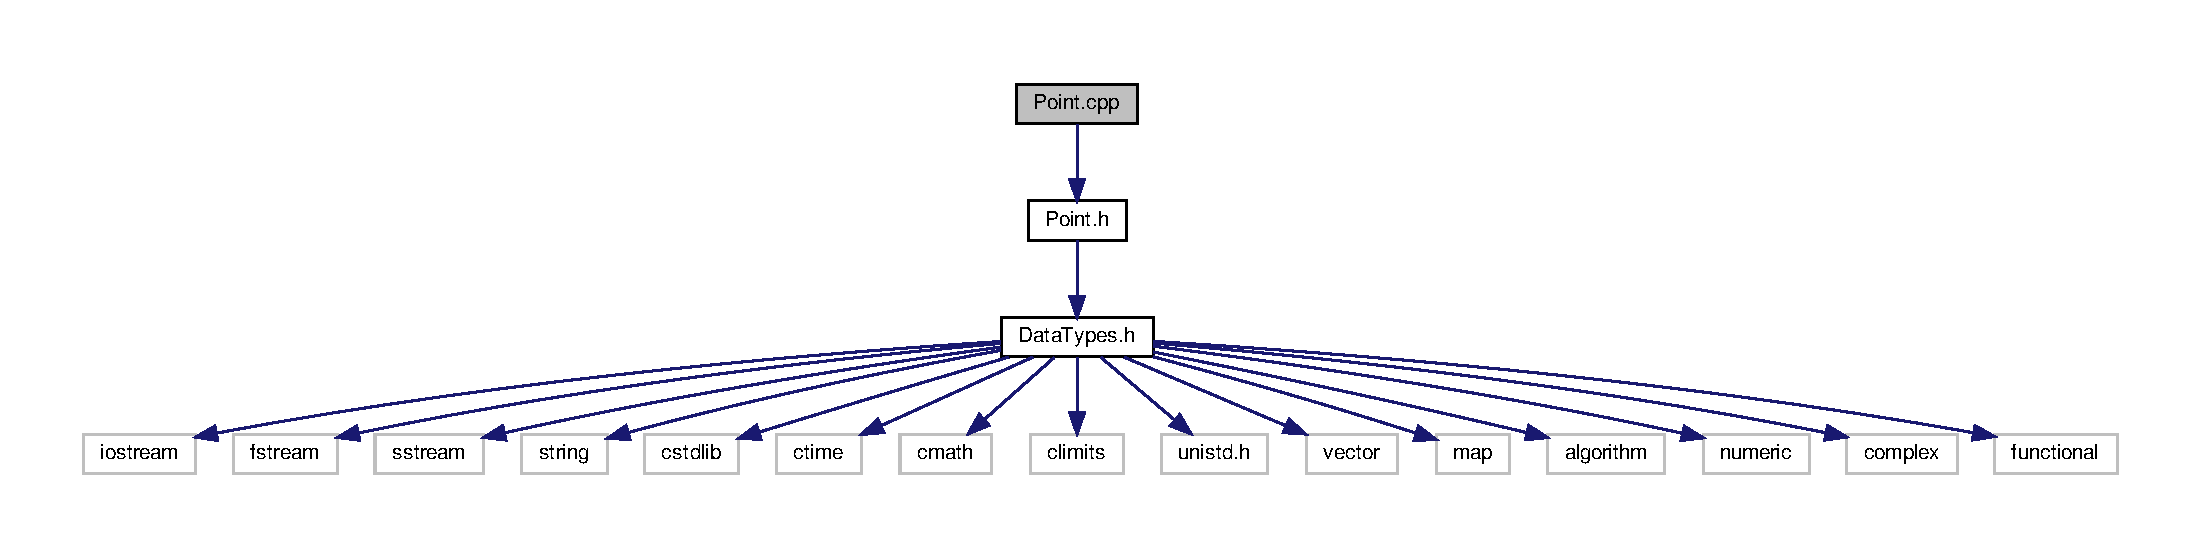
\includegraphics[width=350pt]{_point_8cpp__incl}
\end{center}
\end{figure}

\section{Point.\+h File Reference}
\label{_point_8h}\index{Point.\+h@{Point.\+h}}
{\ttfamily \#include \char`\"{}Data\+Types.\+h\char`\"{}}\newline
Include dependency graph for Point.\+h\+:\nopagebreak
\begin{figure}[H]
\begin{center}
\leavevmode
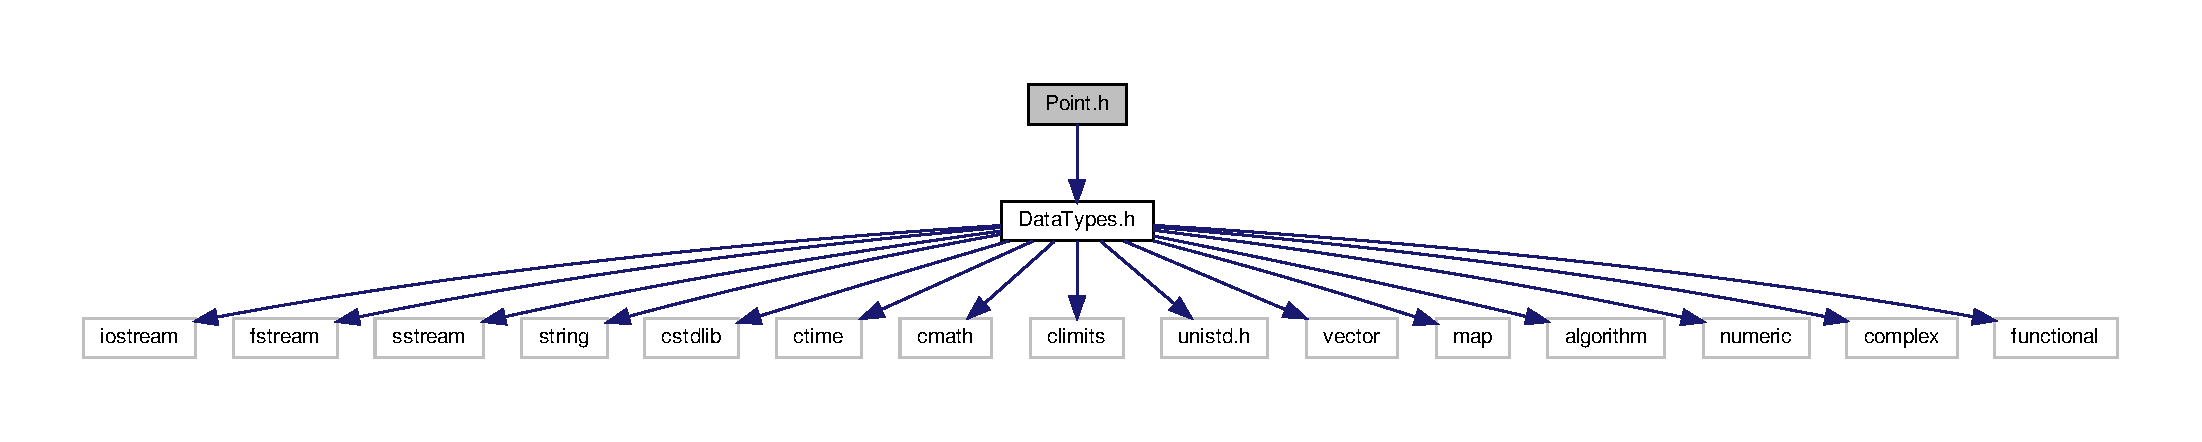
\includegraphics[width=350pt]{_point_8h__incl}
\end{center}
\end{figure}
This graph shows which files directly or indirectly include this file\+:\nopagebreak
\begin{figure}[H]
\begin{center}
\leavevmode
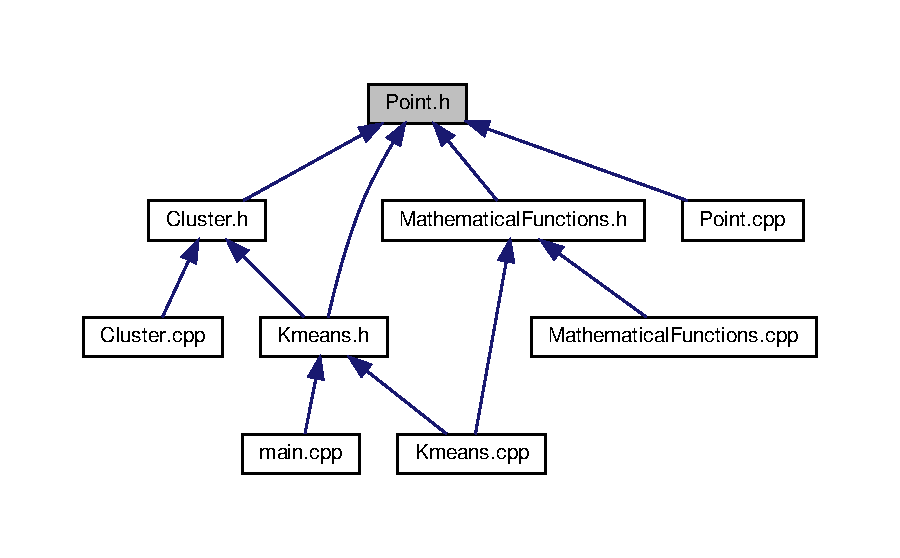
\includegraphics[width=350pt]{_point_8h__dep__incl}
\end{center}
\end{figure}
\subsection*{Classes}
\begin{DoxyCompactItemize}
\item 
class \textbf{ Point}
\end{DoxyCompactItemize}

\section{Properties\+Parser.\+cpp File Reference}
\label{_properties_parser_8cpp}\index{Properties\+Parser.\+cpp@{Properties\+Parser.\+cpp}}
{\ttfamily \#include $<$fstream$>$}\newline
{\ttfamily \#include $<$sstream$>$}\newline
{\ttfamily \#include \char`\"{}Properties\+Parser.\+h\char`\"{}}\newline
Include dependency graph for Properties\+Parser.\+cpp\+:\nopagebreak
\begin{figure}[H]
\begin{center}
\leavevmode
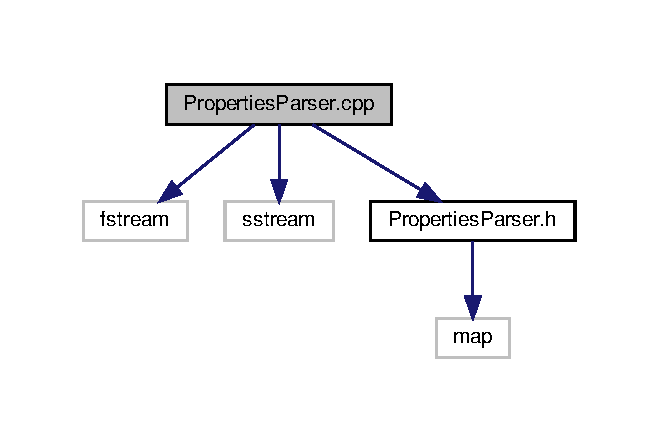
\includegraphics[width=316pt]{_properties_parser_8cpp__incl}
\end{center}
\end{figure}

\section{Properties\+Parser.\+h File Reference}
\label{_properties_parser_8h}\index{Properties\+Parser.\+h@{Properties\+Parser.\+h}}
{\ttfamily \#include $<$map$>$}\newline
Include dependency graph for Properties\+Parser.\+h\+:
\nopagebreak
\begin{figure}[H]
\begin{center}
\leavevmode
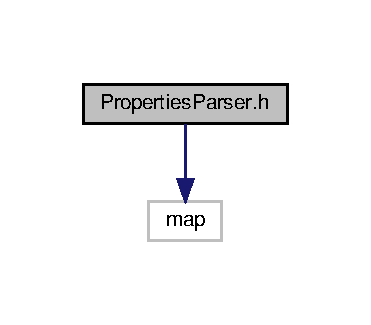
\includegraphics[width=178pt]{_properties_parser_8h__incl}
\end{center}
\end{figure}
This graph shows which files directly or indirectly include this file\+:
\nopagebreak
\begin{figure}[H]
\begin{center}
\leavevmode
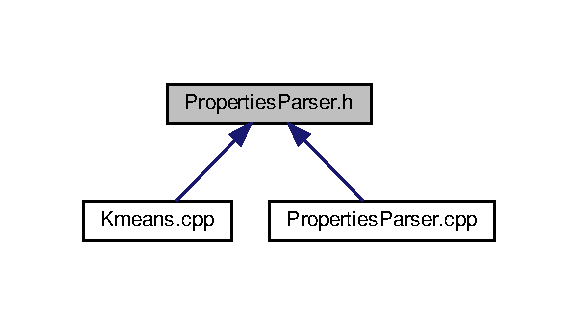
\includegraphics[width=278pt]{_properties_parser_8h__dep__incl}
\end{center}
\end{figure}
\subsection*{Classes}
\begin{DoxyCompactItemize}
\item 
class \textbf{ Properties\+Parser}
\end{DoxyCompactItemize}

\section{R\+E\+A\+D\+M\+E.\+md File Reference}
\label{_r_e_a_d_m_e_8md}\index{R\+E\+A\+D\+M\+E.\+md@{R\+E\+A\+D\+M\+E.\+md}}

%--- End generated contents ---

% Index
\backmatter
\newpage
\phantomsection
\clearemptydoublepage
\addcontentsline{toc}{chapter}{Index}
\printindex

\end{document}
